\documentclass[spanish]{fpunathesis}

\usepackage{babel}
\usepackage[utf8]{inputenc}
\usepackage[T1]{fontenc}
\usepackage{cleveref}
\usepackage{textcomp}
\usepackage[inline,shortlabels]{enumitem}
\usepackage{amsmath}
\usepackage{caption}
\usepackage{color}

\graphicspath{{capitulos/2/figuras/}{capitulos/4/figuras/}{capitulos/6/figuras/}}

\begin{document}

\title{Aproximación colaborativa del tránsito vehicular basado en aplicaciones móviles}
\author{Alfredo Daniel Campuzano Romero \and Rubén Darío López Rojas}
\degree{Informática}
\advisor{Ing.}{Joaquín Quinto Lima Molinari}
\logosource{logo.png}
\maketitle

\tableofcontents
\listoffigures
\listoftables
%\listofalgorithms
%\listofsymbols

\mainmatter
\chapter{Introducción}
\label{cap:1}

\section{Motivación}

La congestión del tránsito es uno de los problemas más serios que enfrentan la mayoría de las zonas urbanas hoy en día, el constante aumento del parque de automóviles, el alto uso de vehículos privados y la falta de planificación de las ciudades son algunos de los factores que afectan negativamente la calidad de vida de los ciudadanos. Además, los países en vías de desarrollado carecen de sistemas de control de tránsito debido al alto costo de inversión requerido y en algunos casos tampoco existen servicios proveídos por empresas privadas para este fin. Esta situación dificulta la utilización eficiente de las vías de tránsito existentes, es por eso que se hace evidente la necesidad de recolectar y analizar información sobre el tránsito de forma barata y sencilla, y que requiera una mínima inversión.

En este trabajo se propone la implementación de un sistema que permita aproximar las condiciones del tránsito utilizando información proveída por dispositivos móviles en tiempo real. Para ello se estudia el estado del arte de las técnicas de recolección, análisis y distribución de información, y se seleccionan los mecanismos más adecuados a las necesidades y limitaciones del medio. Dicha información debe quedar disponible de forma pública para ser utilizada de modo a desarrollar soluciones que ayuden a mitigar la problemática de la congestión vehicular.

\section{Justificación y Antecedentes}

Debido a que los países en vías de desarrollo no cuentan con infraestructura vial bien planificada y  tampoco con tecnología instalada para monitorear el estado del tráfico, se hace necesario buscar una alternativa económica para obtener información precisa y confiable, que permita aproximar la situación actual del tránsito en tiempo real. Es así, que los sistemas de información de tráfico basados en \emph{Floating Car Data} (FCD) han demostrado ser una alternativa viable para obtener esta información de forma económica y eficiente \cite{schafer2002traffic,reinthaler2007evaluation}.

Los sistemas existentes de FCD se basan en la utilización de vehículos sonda equipados con sensores GPS. Para este propósito se han utilizado flotas de taxis \cite{schafer2002traffic,reinthaler2007evaluation} y sistemas instalados por empresas de seguro en los vehículos de sus clientes \cite{giovannini2011novel}. Sin embargo en países menos desarrollados no existen programas o iniciativas públicas y/o privadas que promuevan la utilización de este tipo de sistemas.

Por otra parte, la utilización de teléfonos móviles inteligentes, equipados con sensores GPS, está creciendo a un ritmo considerable y los automovilistas generalmente llevan consigo este tipo de teléfonos. Es así que surge la posibilidad de utilizar esta tecnología como una forma barata y sencilla de recolectar información para estimar el estado del tránsito. Este tipo de tecnología ya se ha utilizado en aplicaciones para el rastreo de vehículos \cite{thiagarajan2010cooperative}, estimación del tiempo de llegada de buses \cite{zhou2012long} y estimación de tiempo de viaje \cite{thiagarajan2009vtrack}. Siguiendo la idea anterior, diversos estudios han demostrado la factibilidad de utilizar esta tecnología para estimar el estado del tráfico en tiempo real \cite{tao2012real,herrera2010evaluation}, sugiriendo que una penetración de entre un 2 y 3\% es suficiente para proporcionar mediciones precisas de la velocidad del flujo del tráfico \cite{herrera2010evaluation}.

Para estimar el estado del tráfico primeramente se debe determinar la trayectoria de los vehículos por las calles de la ciudad, este proceso es conocido por el nombre de \emph{Map Matching} (MM). Existe una gran variedad algoritmos de MM, desde lo más sencillos, basados solamente en información geográfica \cite{white2000some}, hasta los más complejos basados en modelos estadísticos y otras técnicas avanzadas \cite{quddus2006high,kim2001adaptive}. Debido a las limitaciones impuestas por las plataformas móviles (uso de batería, conectividad limitada, entre otros) que se utilizan para obtener los datos, este trabajo se enfoca principalmente en la utilización de algoritmos especializados en procesar muestras relativamente dispersas y poco precisas \cite{lou2009map}.

Con el objetivo de distribuir la información de tráfico, muchos sistemas actualmente se basan en la formación de redes ad-hoc entre los dispositivos móviles \cite{zhong2008disseminating,leontiadis2011effectiveness}. Esto dificulta que los datos obtenidos sean procesados de forma adecuada y distribuidos a otros posibles usuarios que se encuentren fuera de estas redes ad-hoc. En este trabajo se propone una arquitectura centralizada de manera a que todo el procesamiento de la información y la distribución de la información sean manejados por un servidor dedicado.

Existen implementaciones comerciales y/o libres similares a la solución propuesta, sin embargo estos productos generalmente no se encuentran disponibles en los países en vías de desarrollo y además en la literatura no existen trabajos que presenten todos los detalles de diseño, arquitectura y resolución de cuestiones implementativas a la problemática estudiada. Los trabajos anteriores se enfocan generalmente en una sola parte de la problemática, ya sea en la recolección de datos, el análisis o la distribución de la información de tránsito, dejando de lado el estudio de la arquitectura completa de los sistemas.

De esta forma se pretende contribuir al estado del arte al realizar un estudio completo de las técnicas utilizadas en la implementación de sistemas de información de tránsito, abarcando cada una de las partes involucradas, desde la recolección hasta la distribución de la información, y para cada parte, estudiando y aplicando las técnicas más apropiadas publicadas en el estado del arte.

\section{Objetivos}

El principal objetivo de este proyecto es construir un sistema que permita recolectar y procesar información del estado del tránsito vehicular a través de dispositivos móviles para aproximar el estado del tráfico en tiempo real.

Entre los objetivos específicos se puede citar:

\begin{itemize}

\item Estudiar el estado del arte de las técnicas de recolección de datos de tránsito con un enfoque particular en el área de FCD.

\item Estudiar el estado del arte en técnicas de MM utilizadas para procesar la información obtenida.

\item Estudiar el estado del arte de técnicas de distribución de la información entre dispositivos móviles.

\item Diseñar la arquitectura para un sistema que utilice las técnicas estudiadas de modo a recolectar, analizar, distribuir y utilizar la información del estado del tránsito vehicular.

\item Implementar una aplicación móvil que permita recolectar datos de ubicación de los usuarios, distribuir la información de tránsito procesada y brindar soporte a los usuarios.

\item Implementar un sistema centralizado capaz de recibir los datos de ubicación de los usuarios para determinar el estado del tránsito vehicular.

\end{itemize}

\section{Organización}

El resto del presente trabajo se encuentra organizado de la siguiente forma. En el \Cref{cap:2} se presentan conceptos básicos sobre Sistemas de Información Geográfica y bases de datos espaciales.

El \Cref{cap:3} describe el estado del arte de las técnicas de recolección de datos, con un especial enfoque en las técnicas de FCD basadas en la utilización de dispositivos móviles. 

En el \Cref{cap:4} se realiza un extenso análisis del estado del arte de los algoritmos de MM utilizados para el procesamiento de la información recolectada.

En el \Cref{cap:5} se explican los parámetros, fórmulas y análisis realizados para derivar el estado del tráfico.

El \Cref{cap:6} describe detalladamente la arquitectura de la solución propuesta, las técnicas seleccionadas para la recolección y el análisis de datos, y los algoritmos utilizados en cada paso del proceso.

En el \Cref{cap:7} se presentan las pruebas realizadas y se realiza un análisis de los resultados para verificar el funcionamiento del sistema.

Finalmente en el \Cref{cap:8} se presentan las conclusiones y se proponen trabajos futuros que pueden ser llevados a cabo a partir de éste.

\chapter{Sistemas de Información Geográfica}
\label{cap:2}

Se conocen como Sistemas de Información Geográfica (\emph{Geographic Information Systems} - GIS) a aquellos sistemas basados en computadoras diseñados para la recolección, mantenimiento, análisis y distribución de datos e información geográfica \cite{bolstad2005gis}. Un GIS es un sistema de hardware, software, personas, datos, organización y mecanismos institucionales para recoger, almacenar, analizar y difundir información geográfica \cite{longley2005geographic}.

Los GIS ayudan en el análisis y la toma de decisiones basadas en información geográfica y son aplicables en diversas áreas de la actividad humana como la planificación para el desarrollo de zonas urbanas y rurales, la delimitación de propiedades y el cobro de  impuestos, el análisis del flujo del tráfico en ciudades, etc. En este capítulo se explican los conceptos fundamentales que sirven de base para el desarrollo del GIS propuesto en este trabajo.

\section{Datums y Coordenadas Geográficas}

La tarea fundamental de cualquier GIS es conocer e identificar de forma precisa la ubicación de los objetos de interés dentro de un mapa. En esta sección describimos los principios básicos que permiten definir esta ubicación y representarla en el mapa.

\subsection{Sistemas de Coordenadas}
\label{sistema_de_coordenadas}

El primer paso para definir la ubicación de los objetos es establecer el sistema de coordenadas a utilizar. Se denominan como \emph{coordenadas} al conjunto de números que identifican de forma única a una posición dentro de un sistema de coordenadas. Estos números son representados generalmente como pares $x$,$y$ en un plano cartesiano, o como valores de \emph{latitud} y \emph{longitud} en un sistema de coordenadas geográficas. Para definir el sistema de coordenadas geográficas se tienen en cuenta dos elementos principales: \begin{enumerate*}[1)] \item el tamaño y la forma de la Tierra y \item un conjunto de elementos de referencia a partir de los cuales se puede determinar la ubicación de cualquier otro objeto en la superficie de la Tierra\end{enumerate*}.

La Tierra es modelada como un elipsoide achatado hacia los polos cuyo semieje mayor corresponde al radio en la dirección del ecuador y cuyo semieje menor corresponde al radio en la dirección de los polos. Los polos están definidos por el eje de rotación del elipsoide y el ecuador se define como el círculo a mitad de camino entre los dos polos, en un ángulo recto con respecto al eje polar, y que cubre la dimensión más ancha de la elipsoide (Ver \Cref{fig:elipsoide}).

\begin{figure}[h]
	\centering
	\input{capitulos/2/figuras/figura1.pdf_tex}
	\caption[Elipsoide que modela la superficie de la Tierra]{Elipsoide utilizado para modelar la superficie del planeta Tierra}
	\label{fig:elipsoide} 
\end{figure}

Los sistemas de coordenadas geográficas se componen de la \emph{latitud}, que varía de norte a sur, y la \emph{longitud}, que varía de este a oeste. Las líneas de longitud constante son denominadas \emph{meridianos}, y las líneas de latitud constante son denominadas \emph{paralelos}. Los paralelos son líneas paralelas entre sí en dirección este-oeste alrededor de la Tierra. Los meridianos son líneas que van de sur a norte y convergen en los polos. Por convención, el ecuador se toma como la latitud cero y las latitudes al sur y al norte varían en un rango de hasta 90°. Se toma como longitud cero al meridiano que atraviesa el Observatorio Real de Greenwich, en Inglaterra y las longitudes al este u oeste se especifican como ángulos de giro con respecto al meridiano de Greenwich, variando de -180° (oeste) a 180° (este) (Ver \Cref{fig:coordenadas}).

\begin{figure}[h]
	\centering
	\input{capitulos/2/figuras/figura2.pdf_tex}
	\caption[Sistema de coordenadas de latitud y longitud]{Sistema de coordenadas de latitud y longitud}
	\label{fig:coordenadas} 
\end{figure}

\subsection{Datums geodésicos}

%TODO explicar qué es Geodesia.

Con el sistema de coordenadas definido se procede a estimar las longitudes y latitudes de todas las demás ubicaciones a través de mediciones. Mediante estas estimaciones se establecen un conjunto de puntos de referencia para los cuales la latitud y la longitud han sido precisamente determinadas. Todas las demás coordenadas se miden en referencia a este conjunto de puntos. El conjunto de puntos resultante se conoce como \emph{datum geodésico}.  Un datum geodésico consta de dos componentes principales. El primer componente es un elipsoide con un sistema de coordenadas esféricas o cartesianas de tres dimensiones y un origen. La segunda parte consiste en un conjunto de puntos y líneas cuyas coordenadas han sido medidas cuidadosamente utilizando los mejores métodos y equipos \cite{bolstad2005gis}.

A lo largo de la historia diferentes estudios han determinado diversos valores para los radios y el centro del elipsoide. Debido a errores de medición, diferencias en los métodos de cálculo y a que la tierra no es un elipsoide perfecto, diferentes estimaciones alrededor del mundo tienen ligeramente diferentes orígenes, ejes de orientación y radios. Estas diferencias aunque pequeñas, generalmente resultan en estimaciones bastante diferentes para las coordenadas de una misma localización, dependiendo del elipsoide utilizado. En la actualidad las mediciones globales y la avanzada capacidad computacional permiten estimar elipsoides aplicables de forma global.

El primer datum utilizado ampliamente en Norteamérica fue el \emph{North American Datum} de 1927 (NAD27), su sucesor fue el \emph{North American Datum} de 1983 (NAD83), las mejores estimaciones de las localizaciones de los puntos cambiaron en hasta 200 metros entre estos dos datums. En la \Cref{fig:datum-latitud} se puede apreciar el desplazamiento de la latitud entre los datums NAD83 y NAD27 y en la \Cref{fig:datum-longitud} se visualiza la diferencia de longitud entre los mismos. El \emph{World Geodetic System} de 1984 (WGS84) es un conjunto de datums globales desarrollado y utilizado principalmente por el Departamento de Defensa de los Estados Unidos y hoy en día es ampliamente aceptado y utilizado en todo el mundo \cite{longley2005geographic}.

\begin{figure}[h]
	\centering
	\input{capitulos/2/figuras/figura3.pdf_tex}
	\caption[Desplazamiento de la latitud entre NAD83 y NAD27]{Desplazamiento de la latitud de los datums en metros, NAD83 menos NAD27}
	\label{fig:datum-latitud} 
\end{figure}

\begin{figure}[h]
	\centering
	\input{capitulos/2/figuras/figura4.pdf_tex}
	\caption[Desplazamiento de la longitud entre NAD83 y NAD27]{Desplazamiento de la longitud de los datums en metros, NAD83 menos NAD27}
	\label{fig:datum-longitud} 
\end{figure}

%\subsection{Proyecciones}

%Una \emph{proyección} es una representación sistemática de las posiciones de la superficie curva de la Tierra sobre una superficie plana de un mapa. El mapa resultante sufre una distorsión debido a la traducción de una superficie curva a una plana. La proyección puede definirse por lo tanto como la transformación de una posición en la superficie de la Tierra, identificada por su latitud y longitud $(\varphi,\lambda)$ a una posición en coordenadas cartesianas $(x,y)$. Cualquier proyección puede representarse como un par de funciones matemáticas: \begin{displaymath} x=f(\varphi,\lambda );\quad y=g(\varphi,\lambda ) \end{displaymath}

%Las proyecciones se pueden clasificar de acuerdo a su forma, en \emph{cónicas}, \emph{cilíndricas} o \emph{planas} (ver \Cref{fig:tipos-proyecciones}) y de acuerdo a su orientación en \emph{ecuatoriales}, cuando el eje de la proyección coincide con los polos, o \emph{transversales}, cuando coincide con el ecuador.

%\begin{figure}[h]
%	\centering
%	\input{capitulos/2/figuras/figura5.pdf_tex}
%	\caption[Tipos de proyecciones por forma]{Tipos de proyecciones: a) cilíndrica, b) cónica y c) plana}
%	\label{fig:tipos-proyecciones} 
%\end{figure}

%Algunas de las proyecciones más importantes son la Proyección Cilíndrica Equidistante; la Proyección Conforme de Lambert (cónica), la Proyección Transversa de Mercator (cilíndrica) y el Sistema de Coordenadas Universal Transversal de Mercator (UTM por sus siglas en Inglés), que está basada en la Proyección Normal de Mercator pero en lugar de ser tangente al ecuador es tangente a un meridiano.

\section{Modelos de datos}

Los fenómenos geográficos requieren de dos características para representar el mundo real; \emph{qué} se está representando, y \emph{dónde} está. Para lo primero comúnmente utilizamos conceptos como `ciudad', `calle', `río', etc. Los modelos de datos geográficos son los equivalentes formales de estos modelos conceptuales y definen las estructuras de datos abstractas que serán almacenadas en las bases de datos espaciales y manipuladas por el GIS \cite{burrough1998principles}.

\subsection{Modelo de Datos Vectorial}

En un modelo vectorial cada objeto del mundo real es representado como uno de tres posibles tipos de datos geométricos: \emph{puntos}, \emph{líneas} o \emph{polígonos} (ver \Cref{fig:modelo-vectorial}). Un punto se representa de forma única por sus coordenadas (ciudades, puestos de salud, comisarías), las líneas se representan como una lista ordenada de coordenadas correspondientes a sus vértices (rutas, ríos y arroyos) y los polígonos se representan como uno o más segmentos de líneas que se cierran para formar una figura delimitada (propiedades rurales, lagos, distritos). Las coordenadas que definen la geometría de cada objeto pueden tener 2, 3, 4 o más dimensiones. En algunos modelos de datos las figuras geométricas pueden ser representadas por curvas definidas por una función matemática (ej. curvas de Biézer).

\begin{figure}[h]
	\centering
	\input{capitulos/2/figuras/figura7.pdf_tex}
	\caption{Modelo de datos vectorial}
	\label{fig:modelo-vectorial} 
\end{figure}

Objetos del mismo tipo (ej. calles) normalmente son guardados en una tabla de base de datos en la que cada objeto ocupa una fila de la tabla y cada atributo del objeto corresponde a una columna de la tabla. En un GIS también se puede almacenar información topológica sobre los objetos, por ejemplo las relaciones de adyacencia y conectividad entre las calles o su sentido de circulación y su límite de velocidad.

\subsection{Modelo de Datos Raster}

%TODO agregar un footenote a la palabra "raster" con un link a Wikipedia por ej.

En una representación \emph{raster} el espacio es dividido en una colección de celdas rectangulares, todas las variaciones geográficas son expresadas asignando propiedades o atributos a estas celdas. Este tipo de representación requiere que la superficie curva de la tierra sea proyectada en una superficie plana. Debido a que esto genera distorsiones, las celdas en una representación \emph{raster} no son perfectamente iguales en forma o área a la superficie que representan. Cuando se usa este formato, toda la información acerca de las variaciones dentro de una celda es perdida y se asigna un único valor a toda la celda (Ver \Cref{fig:modelo-raster}).

\begin{figure}[h]
	\centering
	\input{capitulos/2/figuras/figura8.pdf_tex}
	\caption{Modelo de datos raster}
	\label{fig:modelo-raster} 
\end{figure}

Las celdas pueden contener atributos basados en diversos esquemas de codificación. Por ejemplo, un esquema de codificación simple puede asignar un valor binario, cero o uno, a cada celda para representar la presencia o ausencia de forestación en dicha celda. Múltiples atributos pueden ser guardados para cada celda en una tabla en la que cada columna es un atributo de la celda y cada fila representa a una celda en particular. Los datos usualmente son guardados en archivos comprimidos o en bases de datos relacionales.

\subsection{Modelos de Datos de Red}

El modelo de red es un tipo especial de modelo topológico que puede ser utilizado para modelar el flujo de bienes y servicios. En un GIS las redes son modeladas como puntos o nodos (ej. intersecciones de calles, fusibles, interruptores, válvulas de agua) y líneas (calles, líneas de transmisión y tuberías). Las relaciones topológicas de la red definen cómo las líneas se conectan entre sí en los nodos y también pueden definir reglas sobre cómo los flujos pueden moverse a través de una red.

Por ejemplo, en una red de calles que está compuesta por un conjunto de nodos (intersecciones de las calles) y líneas (las calles), así como las relaciones topológicas entre las mismas (restricciones de giro en los nodos, sentido de las calles, límites de velocidad), la información topológica permite analizar el flujo de tráfico a través de la red y determinar los puntos más congestionados o calcular caminos más cortos de un punto de la red a otro.

\subsection{Red Irregular de Triángulos (TIN)}

Los modelos de datos geográficos descritos hasta ahora se utilizan para representar datos en una o dos dimensiones. Para representar superficies tridimensionales en un GIS se pueden utilizar modelos \emph{raster} o redes irregulares de triángulos (\emph{Triangulated Irregular Network} - TIN). En los modelos \emph{raster} cada celda almacena la altura de la superficie en una localización dada. En una estructura TIN se representa una superficie como una serie de elementos triangulares contiguos que no se superponen entre sí.

Un TIN es una estructura topológica que almacena información acerca de los nodos que conforman cada triángulo y sus triángulos vecinos. El triángulo está representado por una secuencia de tres nodos, cada nodo está definido por sus coordenadas $x$, $y$, $z$ (Ver \Cref{fig:modelo-tin}). Los triángulos tienen como atributos su pendiente, orientación y área, los vértices tienen atributos de elevación y los bordes tienen como atributos su pendiente y dirección. Al igual que en los demás modelos de datos, cada triángulo puede tener otros datos o atributos asociados.

\begin{figure}[h]
	\centering
	\input{capitulos/2/figuras/figura9.pdf_tex}
	\caption{Red irregular de triángulos}
	\label{fig:modelo-tin} 
\end{figure}

\section{Bases de Datos Espaciales}

Una base de datos espacial es aquella en la que están definidos tipos de datos especiales para representar objetos geométricos y permite guardar estos objetos, que usualmente son de origen geográfico, en tablas regulares de una base de datos. Además provee funciones e índices para consultar y manipular estos datos \cite{obe2011postgis}. Las bases de datos espaciales no necesitan ser relacionales pero muchas de las más populares lo son.

En las bases de datos espaciales se definen tipos de datos que representan puntos, líneas y polígonos a partir de los cuales se pueden construir otros tipos de datos más complejos y representar objetos del mundo real. Estas bases de datos están especialmente diseñadas para representar información en dos dimensiones en formato vectorial, pero también pueden almacenar datos \emph{raster} y topologías tridimensionales.

\subsection{Análisis, procesamiento y consultas espaciales}

%TODO footnote para PostGIS y Oracle Spatial

Una consulta espacial en una base de datos es aquella que utiliza funciones geométricas para responder preguntas acerca del espacio y de los objetos en el espacio. Extensiones para bases de datos relacionales tales como PostGIS y Oracle Spatial agregan un conjunto de funciones a las ya existentes en el lenguaje SQL estándar que trabajan con objetos geométricos de forma similar a cómo las funciones estándar trabajan con los tipos de datos nativos de la base de datos.

Por ejemplo, existen funciones que indican la cantidad de tiempo que hay entre dos fechas o si una fecha dada corresponde al pasado o al futuro. De forma similar las bases de datos espaciales proveen funciones que permiten obtener la distancia entre dos figuras geométricas, o el área total de un polígono. Las funciones espaciales también permiten crear y modificar objetos geométricos.

%TODO footnote para OGC

Actualmente existen estándares que definen este conjunto de tipos de datos y funciones espaciales mínimas para una base de datos GIS. El \emph{Open Geospatial Consortium} (OGC) es un consorcio internacional de la industria cuyo objetivo es tratar de estandarizar la forma en que los datos geométricos y espaciales son accedidos y distribuidos. OGC cuenta con numerosas especificaciones que definen el acceso a los datos geoespaciales, servicios web para consulta y manipulación de datos, formatos de datos geoespaciales y consulta de datos geoespaciales.

\subsection{Productos comerciales y de código abierto}

%TODO footnote para SQLite, MySQL, SQL Server, PostGIS

Existen varias bases de datos espaciales disponibles en el mercado que implementan los estándares OGC, tanto de código abierto como soluciones comerciales. Entre las bases de datos de código abierto más populares podemos citar a SpatialLite/SQLite, PostgreSQL/PostGIS y MySQL. Los productos comerciales más populares incluyen a Oracle Spatial y SQL Server de Microsoft.

PostGIS es una extensión para PostgreSQL que agrega soporte para tipos de datos geométricos y funciones espaciales convirtiendo a PostgreSQL en una base de datos espacial. PostGIS es un proyecto de código abierto que se publica bajo la Licencia Pública General de GNU. Además de los tipos de datos básicos provee otros tipos de datos más complejos como multi-polígonos, multi-puntos, multi-líneas y curvas geométricas. PostGIS 2 además agrega soporte para datos \emph{raster} y datos tridimensionales en formato TIN. De forma similar SpatialLite es una extensión para SQLite que agrega soporte para tipos de datos y funciones geométricas.

Oracle Spatial es una extensión para la base de datos Oracle que proporciona tipos de datos y funciones para la gestión de datos espaciales. Los tipos estándar y funciones de Oracle (CHAR, DATE, INTEGER, etc) se extienden con equivalentes geográficos. Oracle Spatial provee tres tipos básicos de figuras geométricas: puntos, líneas y polígonos (incluyendo polígonos complejos con agujeros), a partir de los cuáles se pueden construir estructuras de datos más complejas. Además, Oracle Spatial puede almacenar y administrar datos de tipo \emph{raster}.

\chapter{Recolección de datos de tráfico}

Actualmente existen una variedad de tecnologías para la recolección automática de datos del tráfico. Según \cite{mimbela2003summary} podemos dividir estas tecnologías en dos métodos. El primero, es la tecnología In-Situ, que toma los datos del tráfico a través de detectores a lo largo del camino. Generalmente estas tecnologías de conteo de tráfico pueden dividirse en dos categorías: la intrusiva y la no intrusiva. Por el otro lado tenemos los datos de vehículo flotante (FCD por sus siglas en inglés). FCD es una alternativa para obtener datos del tráfico de gran calidad y se está volviendo crucial para el desarrollo de nuevos Sistemas Inteligentes de Transporte (ITS por sus siglas en inglés).

\section{Tecnologías In-Situ}

En \cite{klein2006traffic} se puede apreciar un gran número de sensores fijos para la detección del tráfico. Estas tecnologías de detección In-Situ se dividen en dos categorías: tecnologías intrusivas, que están montadas en o por debajo de la superficie de las rutas y cuya instalación ocasiona la interrupción potencial del tráfico. En contrapartida, las tecnologías no intrusivas son montadas en o por encima de la superficie de las rutas, su instalación no genera interrupción del tráfico o lo hace en pequeña medida. 

\subsection{Tecnologías Intrusivas}

Los tipos de sensores y la ubicación de los mismos se pueden observar en la \Cref{fig:intrusiva}. El primer tipo de unidades son los Sensores Magnéticos Pasivos o magnetómetros que pueden ser montados de forma permanente en hoyos a lo largo del camino, o pegados a la superficie de la ruta. Estas unidades se comunican a una estación de procesamiento cercana, ya sea utilizando cables debajo del camino, o a través de comunicación inalámbrica. El sensor tiene una zona circular o elíptica de alcance de detección. Los magnetómetros monitorean la fluctuación en la fuerza del campo magnético, el cual cambia en presencia de objetos de metal moviéndose (automóviles).

\begin{figure}[h]
	\centering
	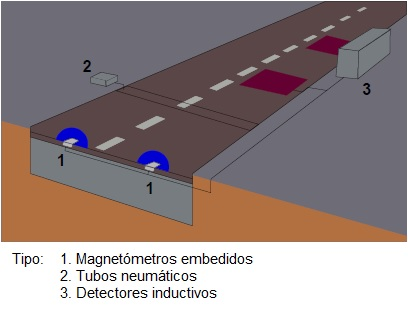
\includegraphics[width=0.7\textwidth]{capitulos/3/figuras/figura1.jpg}
	\caption{\label{fig:intrusiva} Típicas configuraciones de detección intrusiva}	
	%TODO cambiar el texto 3 del gráfico por Detectortes de inducción %
\end{figure}

El segundo tipo de unidades utilizan tubos neumáticos que son extendidos a través de la calzada y se fijan en el lado de la acera en ambos extremos. Estos sistemas solamente se pueden implementar de forma temporal, debido a la naturaleza frágil de los tubos, que son fácilmente dañados por vehículos pesados o que se mueven a gran velocidad. Estos sensores envían una ráfaga de presión de aire a lo largo de un tubo de goma cuando un vehículo pasa por encima de los tubos. El pulso de presión de aire cierra un interruptor de aire, produciendo una señal eléctrica que es transmitida a un contador. Tienen la ventaja de ser sistemas portables utilizando ácido-plomo, gel, u otras baterías recargables como fuente de energía.

El tercer tipo son los Detectores de Bucle de Inducción (IDL por sus siglas en inglés). Consisten en rollos de alambre recubierto, enterrados en ranuras cortadas en la superficie de la carretera y sellados con masilla bituminosa. Los datos son enviados a través de un cable enterrado con los bucles hasta una unidad de procesamiento al borde de la carretera. La zona de detección para los sensores de bucle de inducción depende de la forma de corte de la ranuras del bucle. Los IDL son una tecnología barata y madura. La oscilación de la señal eléctrica es aplicada al bucle, el metal contenido en el chasís de un vehículo en movimiento cambia las propiedades eléctricas del circuito. Estos cambios son detectados por una unidad al costado del camino, que disparan un evento de vehículo.

El cuarto tipo de sistemas intrusivos es Weigh-In-Motion (WIM) mostrado en \Cref{fig:Weight-In-Motion}, los detectores consisten en un sensor piezoeléctrico ubicado en un canal a través del camino. El sistema registra la tensión medida por los sensores y calcula la carga dinámica, la carga estática se calcula utilizando la carga dinámica y parámetros de calibración. Los parámetros de calibración dependen de factores como la velocidad del vehículo y el pavimento o la dinámica de suspensión que influencia en los cálculos de la carga estática. La precisión de los sistemas WIM puede ser expresada como función a la velocidad con que el vehículo pasa sobre las placas, asumiendo que el sistema está instalado en una carretera sujeta a las condiciones normales de tráfico. Estos sistemas son raros y se utilizan en ubicaciones específicas mayormente para el control de acceso.

\begin{figure}[h]
	\centering
	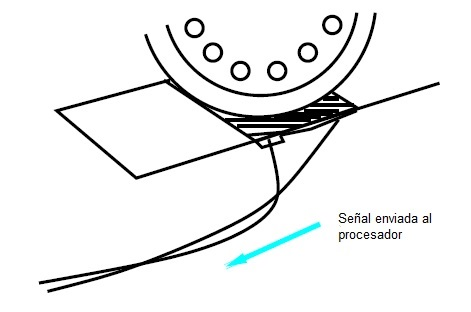
\includegraphics[width=0.7\textwidth]{capitulos/3/figuras/figura2.jpg}
	\caption{\label{fig:Weight-In-Motion}  Sistema de detección Weight-In-Motion}	
\end{figure}

\subsection{Tecnologías No Intrusivas.}

Las tecnologías no intrusivas incluyen recolección de datos por video, detectores infrarrojos pasivos o activos, radares de microondas, detectores ultrasónicos, detectores acústicos, detectores láser y fotografía aérea. Según \cite{mathew2014transportation}, todas estas tecnologías representan campos emergentes que se están expandiendo rápidamente con continuos avances en el procesamiento de señales. Actualmente estas tecnologías son utilizadas para proveer información suplementaria para lugares seleccionados o para aplicaciones específicas. La mayoría de los sistemas no intrusivos son operacionalmente y visualmente similares, consistiendo en pequeñas unidades electrónicas montadas en contenedores a prueba de agua y colocadas en varias ubicaciones como se puede observar en la \Cref{fig:noIntrusica}.

\begin{figure}[h]
	\centering
	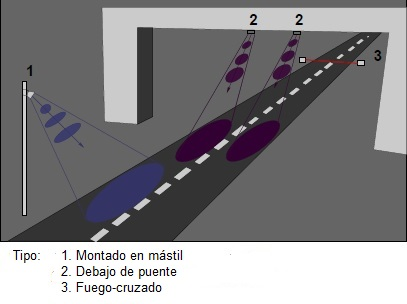
\includegraphics[width=0.7\textwidth]{capitulos/3/figuras/figura3.jpg}
	\caption{\label{fig:noIntrusica}  Configuraciones típicas de tecnologías no intrusivas}	
\end{figure}

El primer tipo de detectores no intrusivos son los montados al costado de la carretera. El detector procesa un campo de visión que cubre un área oblicua, ya sea por encima o por debajo de la unidad. También existen múltiples zonas de detección definidas dentro del campo de visión, dependiendo del tipo de detector específico y la tecnología utilizada.

Problemas de oscurecimiento ocurren cuando vehículos grandes cubren a vehículos pequeños del detector o cuando el campo de visión es muy grande, causando la detección de vehículos fuera del carril deseado. El segundo tipo de detectores no intrusivos son montados debajo de puentes o portales, con un campo de visión justo por debajo de los mismos, o ligeramente oblicuo a la unidad. Finalmente, algunas unidades como los monitores de polución de camino abierto son montadas a nivel del piso a los lados del camino, disparando un haz a través de la carretera. Estas unidades están sujetas al enmascaramiento de lado a lado, por lo tanto, son más adecuadas para un solo carril.

En la detección por imagen de video los parámetros del tráfico son recolectados a través del análisis cuadro por cuadro de las imágenes capturadas por las cámaras al costado del camino. Dependiendo de la tecnología de procesamiento, se pueden obtener prácticamente todos los parámetros del tráfico a través de análisis de video. Un problema con este sistema es que es susceptible al oscurecimiento y su rendimiento puede decaer con el mal clima o con bajas condiciones de luz.

Los sensores infrarrojos pueden ser montados por encima o al costado del tráfico dependiendo de la información que se quiera obtener con ellos. Estos sensores son utilizados para obtener el volumen, la velocidad y el tipo de vehículos. Tienen la ventaja de ser menos susceptibles al mal clima. Cuando los sensores poseen una baja resolución la precisión en la velocidad y el largor de los vehículos tienden a ser bastante imprecisos.

\section{Tecnologías en vehículo o Floating Car Data (FCD)}

En adición a la utilización de tecnologías In-Situ, muchas aplicaciones de gestión de tráfico utilizan dispositivos en los vehículos, generalmente conocidos como sistemas de ubicación automática de vehículo (AVL por sus siglas en inglés). Los dispositivos AVL proveen información de posición cuando un vehículo equipado con ellos pasa cierto punto de la red, o información continua a medida que el vehículo viaja a través de la red. Los anteriores sistemas se basaban en vehículos equipados con transpondedores que transmitían y recibían información de los dispositivos ubicados en la carretera. Los sistemas actuales se basan en la tecnología del Sistema de Posicionamiento Global (GPS por sus siglas en inglés).

El principio de FCD es recolectar datos de tráfico en tiempo real ubicando los vehículos a través de teléfonos móviles o dispositivos GPS en toda la red de caminos como se muestra en la \Cref{fig:ComunicacionGPS}. Todos los vehículos equipados con estos dispositivos actúan como sensores para la red de caminos. Datos como la ubicación del vehículo, la velocidad y dirección del viaje son enviados de forma anónima un un centro de procesamiento. Después de la recolección y extracción, información útil como el estado del tráfico y rutas alternativas pueden ser distribuidas a los conductores del camino. FCD es una alternativa, o más bien, una fuente de información de alta calidad para las tecnologías existentes. Ayuda a mejorar la seguridad, eficiencia y confiabilidad de los sistemas de transporte.

\begin{figure}[h]
	\centering
	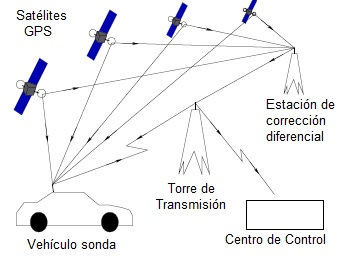
\includegraphics[width=0.7\textwidth]{capitulos/3/figuras/figura4.jpg}
	\caption{\label{fig:ComunicacionGPS}  Comunicación con GPS}	
\end{figure}

\subsection{FCD basado en GPS}

La tecnología GPS se está volviendo cada vez más útil y barata, va en aumento el número de autos equipados con sistemas GPS que le permiten ser ubicados dentro de la red de caminos. La precisión de la ubicación del vehículo es relativamente alta, típicamente menor a 30 metros. Generalmente, los datos del tráfico que se obtienen de vehículos privados o camiones son más adecuados para autopistas y zonas rurales.

Actualmente, los datos de sondas GPS son utilizados como fuente de información en tiempo real por muchos proveedores de servicios pero el limitado número de vehículos equipados y los costos de equipamiento comparados con el FCD obtenido de teléfonos celulares, hacen más atractiva la segunda opción.

\subsection{Identificación por Radiofrecuencia o Sistemas de Transpondedores}

La Identificación por Radiofrecuencia (RFID por sus siglas en inglés)  es un método automático de identificación, que se basa en el almacenamiento y recuperación de datos de áreas remotas utilizando dispositivos llamados etiquetas RFID o transpondedores. La tecnología requiere la cooperación entre lectores y etiquetas RFID. Una etiqueta RFID es un objeto que puede ser aplicado o incorporado a un producto, animal, o persona con el propósito de identificación y seguimiento utilizando ondas de radio. Algunas etiquetas pueden ser leídas desde varios metros de distancia y más allá de la línea de vista del lector.

Una etiqueta RFID se compone de un microchip para recolectar información y de una antena que transmite estos datos de forma inalámbrica a un lector. En su forma más básica, el chip contendrá un identificador serializado, o el número de matrícula, que identifica de manera única al objeto.

\subsection{FCD basado en teléfono móviles}

La rápida expansión de los teléfonos inteligentes y los múltiples sensores que poseen los mismos, los convierte en una fuente invaluable para la obtención de FCD. Muchos trabajos se centran en la utilización de dispositivos móviles para la detección del tráfico, la mayoría aprovechando los sistemas de GPS, pero también existen otros que utilizan las redes GSM, WiFi y hasta la tecnología Bluetooth.

Ya en 2007, \cite{fraser2007use} habla de la viabilidad de utilización de dispositivos móviles como alternativa a los métodos típicos de detección de tráfico. En aquel entonces uno de los problemas grandes encontrados era la precisión, ya que se utilizaba la triangulación de antenas (\Cref{fig:triangulacionAntenas}) como método de ubicación, que tiene una precisión entre 50 y 200 metros. Posteriormente, con la llegada de los sistemas GPS a los teléfonos inteligentes se mejoró bastante el problema de la precisión.

\begin{figure}[h]
	\centering
	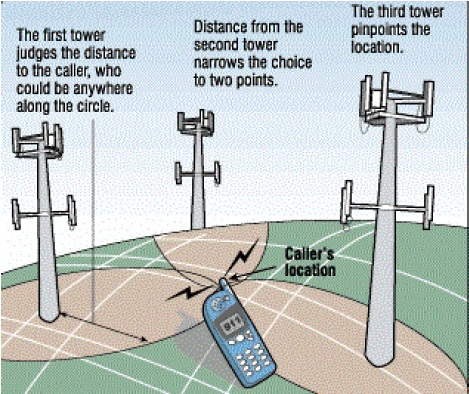
\includegraphics[width=0.7\textwidth]{capitulos/3/figuras/figura5.jpg}
	\caption{\label{fig:triangulacionAntenas} Triangulación de Antenas}	
\end{figure}

A pesar de la baja precisión de los sistemas GSM para la ubicación de dispositivos móviles, se han realizado trabajos como CTrack \cite{thiagarajan2011accurate} que utiliza solamente este método de triangulación de antenas celulares en lugar de GPS o WiFi que bien es sabido consumen un alto nivel de batería. En este método el consumo marginal de energía es cercano a cero. CTrack utiliza un nuevo Modelo Oculto de Markov de dos pasos que secuencia las huellas digitales GSM de los celulares sin convertirlas en coordenadas geográficas, y los fusiona con los datos de los sensores de bajo consumo de energía con los que cuentan la mayoría de los teléfonos inteligentes, incluyendo acelerómetros (para detectar movimiento) y compases magnéticos (para detectar giros). El sistema consiste en dos componentes de software, la librería para el teléfono y el servicio web. La librería recolecta, filtra y escanea los datos obtenidos de GSM y de otros sensores del teléfono y los transmite a través de cualquier red inalámbrica disponible al servicio web, que corre un algoritmo de mapeo de trayectoria sobre los datos recibidos.

Otro trabajo que busca un uso eficiente de energía es EnAcq \cite{fang2011enacq}. El mismo presenta un nuevo método de adquisición de ubicaciones basado en un Map Matching mejorado que se centra en dos desafíos claves: datos imprecisos de trayectoria y consumo de energía. Para mejorar la precisión de los datos de la trayectoria, utiliza un algoritmo mejorado de Map Matching basado en Modelos Ocultos de Markov, que puede encontrar pares candidatos para cada punto sin usar una consulta de rango y determinar la ruta más probablemente seguida por el vehículo. Para evitar el consumo innecesario de energía, utiliza un periodo adaptativo para la toma de ubicaciones por GPS, este periodo de toma de posiciones se basa en el estado de movimiento actual del vehículo.

También existen trabajos que utilizan otros métodos para detectar la ubicación de los vehículos como la tecnología Bluetooth y las redes WiFi \cite{ruppe2012augmenting}, donde se ven enfoques de bajo coste y gran escala para monitorear el tráfico, que aumentan el principio de FCD y permiten la detección de vehículos, transeúntes, ciclistas y pasajeros del transporte público para lograr datos espacio-temporales de tráfico con un aumento considerable de la base de datos subyacente. Este nuevo enfoque se basa en un método para la ubicación anónima a través de la detección indirecta de objetos de tráfico (autos, ciclistas. transeúntes). Esto es ventajoso debido a que varios participantes del tráfico utilizan dispositivos con el WiFi o Bluetooth activado. Por ejemplo, un auto que está equipado con receptores específicos, detecta todos los objetos de tráfico que están dentro de un área a través del número de identificación de WiFi o Bluetooth. Este número de identificación se ve aumentado por las marcas de tiempo y la ubicación de los objetos de detección. Los datos medidos son procesados para obtener las trayectorias, tiempo de viaje, estado del tráfico, matrices de origen-destino y otros parámetros de tráfico.

\section{Sistemas Inteligentes de Transporte (ITS)}

Los Sistemas Inteligentes de Transporte son la aplicación de tecnologías de computación, electrónica y comunicaciones con estrategias de administración de forma integrada para proveer información de viaje para incrementar la seguridad y eficiencia de los sistemas de transporte en las rutas. Estos sistemas incluyen vehículos, conductores, pasajeros, operadores de rutas y administradores, todos interactuando los unos con los otros y enlazándose con la compleja infraestructura de los sistemas para mejorar la seguridad y capacidad de las rutas \cite{chowdhury2003fundamentals}. La arquitectura y el planeamiento de los ITS, que utilizados correctamente mejoran la seguridad y movilidad en el transporte y realzan la conectividad global en términos de mejoras en la productividad logradas a través de la integración de avanzadas tecnologías de comunicación en la infraestructura del transporte.

\subsection{Servicios a usuarios ITS}

Con el fin de implementar ITS, se desarrolla un marco destacando los varios servicios que los ITS pueden proveer a los usuarios. Una lista de 33 servicios a los usuarios ha sido proveída en el plan nacional ITS de los Estados Unidos. El número de servicios de usuario sigue variando con el tiempo cuando un nuevo servicio es añadido. Todos estos servicios están divididos en ocho grupos. La división de estos servicios está basada en la perspectiva de la organización y la distribución de funciones técnicas comunes. Estos ocho grupos de servicios se dividen de la siguiente manera:

\begin{itemize}
\item Gestión de los viajes y el tráfico

\item Operaciones de transporte público

\item Pago electrónico

\item Operaciones de vehículos comerciales

\item Sistemas avanzados de control y seguridad de vehículos

\item Gestión de emergencias

\item Gestión de la información

\item Gestión del mantenimiento y construcción.
\end{itemize}

\subsection{Arquitectura ITS}

La arquitectura de los ITS provee un marco común para planeamiento, definición, e integración de los sistemas inteligentes de transporte. Especifica cómo los diferentes componentes de un ITS deben interactuar entre ellos para ayudar a resolver los problemas del transporte. Proporciona a los profesionales del transporte una gran variedad de opciones para hacer frente a sus necesidades. Identifica y describe varias funciones y asigna responsabilidades a las partes interesadas del ITS. La arquitectura debe cumplir con los siguientes requisitos:
\begin{itemize}
\item Interoperabilidad, la arquitectura debe ser de tal manera que la información recolectada, la función implementada o cualquier equipo instalado pueda ser interoperable por varias agencias de diferentes regiones.

\item Capaz de compartir e intercambiar información. La información de las operaciones de tráfico puede ser útil en los servicios de emergencia.

\item Compartir recursos. torres regionales de comunicación construidas por diversas agencias privadas están obligadas a ser compartidas por las operaciones ITS.
\end{iitemize}


\subsection{Planeamiento ITS}

El planeamiento ITS consiste en integrar ITS en el proceso de planeamiento del transporte. El planeamiento del transporte ayuda a dar forma a un sistema de transporte bien balanceado que pueda cumplir con las demandas futuras. Es un proceso interactivo que incluye identificación de problemas, generación de soluciones, análisis, evaluación e implementación. Esto puede ser integrado con ITS utilizando computadores, sistemas de comunicación y software. Como el planeamiento es realizado normalmente para un periodo largo, la instalación de ITS debe ser actualizable y se debe asegurar que los equipos y tecnologías serán compatibles para futuras mejoras y expansiones.

Los pasos tradicionales en un planeamiento de transporte son los siguientes:

\begin{enumerate}
\item Establecer metas y objetivos

\item Inventario de las condiciones existentes.

\item Análisis de las condiciones existentes.

\item Elementos de largo y corto alcance.

\item Pronóstico del uso de la tierra, población y empleo.

\item Pronóstico de viajes futuros.

\item Desarrollo y evaluación de planes alternativos de transporte.

\item Preparación de planes y programas recomendados.
\end{enumerate}

El proceso de planeamiento de transporte ITS difiere del tradicional, ya que los ITS tienen la capacidad única de integrar diferentes modos de transporte como el transporte público, tráfico, y elementos infraestructurales a través de comunicaciones y control. El potencial de integración multimodal ofrece una gran oportunidad para la planificación a través de los diferentes modos.

\chapter{Map Matching}
\label{cap:4}

Se conoce como \emph{Map Matching} (MM) al proceso de identificar la trayectoria seguida por un vehículo en una red de calles a partir de muestras recolectadas acerca de su ubicación. Este proceso es utilizado en una gran variedad de servicios y aplicaciones GIS, como la predicción de trayectorias de usuarios \cite{eisner2011algorithms}, sistemas de navegación en vehículos \cite{kim2001adaptive}, control del estado del tránsito \cite{thiagarajan2009vtrack}, estimación de llegada de buses \cite{thiagarajan2010cooperative}, entre otros. A continuación se define formalmente el proceso de MM y se presenta un análisis de los algoritmos de MM existentes en la actualidad.

\section{Definición del problema}

Para dar una definición formal del problema de MM deben tenerse en cuenta los siguientes conceptos:

\textbf{Muestra o Punto}: Una muestra o punto es el conjunto de todas las mediciones recolectadas por el vehículo en un instante dado. Estas mediciones incluyen la localización del vehículo, su dirección de desplazamiento, su velocidad, etc.

\textbf{Trayectoria}: Una trayectoria es una secuencia ordenada de muestras o puntos pertenecientes a un vehículo recolectados durante un viaje del mismo.

\textbf{Red de calles}: Una red de calles es un grafo dirigido que representa la forma y las propiedades del sistema de calles de un área geográfica en particular. Los vértices del grafo describen las intersecciones entre las calles y las aristas representan la forma y los atributos de las calles.

\textbf{Camino reconstruido}: Un camino reconstruido es una secuencia ordenada de calles conectadas entre sí a través de las cuáles se infiere que el vehículo pudo haber transitado.

En función a lo anterior, el problema de MM puede definirse de la siguiente forma: \emph{Dada una trayectoria T y una red de calles G, encontrar el camino real R que hace coincidir a T con su reconstrucción más realista sobre G.}

En la \Cref{fig:map-matching} se puede apreciar en rojo la trayectoria de un vehículo sobre una red de calles y en verde el posible camino reconstruido que se infiere el vehículo ha transitado.

\begin{figure}[h]
	\centering
	\input{capitulos/4/figuras/figura41.pdf_tex}
	\caption[Trayectoria y camino reconstruido mediante MM]{Ejemplo de trayectoria (rojo) y camino reconstruido (verde) mediante MM}
	\label{fig:map-matching} 
\end{figure}

\section{Clasificación de algoritmos de MM}

De acuerdo a la información y las técnicas utilizadas para su implementación los algoritmos de MM se pueden clasificar en: \begin{enumerate*}[1)]\item \emph{geométricos}, que utilizan sólo la información de posición y distancia entre las calles y puntos \cite{white2000some}, son sencillos de implementar y suelen utilizarse como paso inicial en la implementación de otros algoritmos; \item \emph{topológicos}, que incorporan información topológica de la red de calles \cite{lou2009map,yuan2010interactive,greenfeld2002matching,quddus2003general}, utilizan información sobre la conectividad, restricciones de giro, sentido y límite de velocidad de las calles; \item \emph{estadísticos}, que definen regiones de probabilidad alrededor de cada punto y analizan los tramos dentro de dichas regiones \cite{ochieng2009map}, estos análisis estadísticos también se utilizan como parte de otros algoritmos, y \item \emph{avanzados}, que combinan diversas técnicas geométricas, topológicas y estadísticas con otros conceptos tales como \emph{Filtros de Kalman}, \emph{Modelos Ocultos de Markov}, \emph{Lógica Difusa}, entre otros \cite{thiagarajan2009vtrack,quddus2006high,thiagarajan2011accurate,fang2011enacq}\end{enumerate*}.

De acuerdo al momento en el que se realiza el procesamiento de los datos, existen dos categorías: \begin{enumerate*}[1)] \item los algoritmos \emph{incrementales} u \emph{on-line}, que realizan el proceso de MM a medida que se van obteniendo nuevos puntos \cite{thiagarajan2009vtrack,thiagarajan2011accurate,greenfeld2002matching,quddus2003general,quddus2006high} y se utilizan en aplicaciones de tiempo real como asistentes personales de navegación, y \item los algoritmos \emph{globales} u \emph{off-line}, que realizan el proceso MM luego de que se han recolectado todos los puntos \cite{lou2009map,yuan2010interactive} y se utilizan en aplicaciones de análisis de tráfico o estudios sobre el comportamiento de usuarios\end{enumerate*}.

Dependiendo de la frecuencia de muestreo se pueden identificar dos categorías más: \begin{enumerate*}[1)] \item los algoritmos para \emph{alta frecuencia} o \emph{high-sampling}, que típicamente trabajan con intervalos de muestra en el rango de los pocos segundos y generalmente se ejecutan de forma \emph{on-line} \cite{greenfeld2002matching,quddus2003general,quddus2006high}, y \item los algoritmos para \emph{baja frecuencia} o \emph{low-sampling},  que funcionan para intervalos de muestreo de varios minutos y se ejecutan generalmente de forma \emph{off-line} \cite{lou2009map,yuan2010interactive}. \end{enumerate*} En general todos los algoritmos pueden ser alimentados con muestras de alta o baja frecuencia pero ciertos algoritmos dejan de ser efectivos a medida que disminuye la frecuencia de muestreo.

\subsection{Algoritmos geométricos}

Los algoritmos geométricos fueron los primeros en ser desarrollados, son los más simples y rápidos pero a la vez son los más propensos a errores. Estos algoritmos tienen en cuenta únicamente la posición de los puntos y de los vértices y aristas que conforman la red de calles \cite{quddus2007current}.

El algoritmo más sencillo se denomina de \emph{punto a punto} \cite{white2000some}, consiste en buscar para cada punto, el vértice dentro de la red de calles que sea el más cercano a dicho punto. Esta técnica es muy propensa a errores puesto que no se tiene en cuenta la conectividad entre los vértices seleccionados e implícitamente favorece a aquellas calles que tengan una mayor densidad de vértices, lo que puede llevar a resultados incorrectos. En la \Cref{fig:punto-a-punto} se puede apreciar cómo el punto $p_0$ es incorrectamente asociado al vértice $b_1$ cuando realmente está más próximo a la línea comprendida entre los vértices $a_0$ y $a_1$.

\begin{figure}[h]
	\centering
	\input{capitulos/4/figuras/figura42.pdf_tex}
	\caption{Error en el algoritmo de punto-a-punto}
	\label{fig:punto-a-punto} 
\end{figure}

Otra técnica utilizada se denomina \emph{punto a curva} \cite{white2000some}, y consiste en buscar para cada punto, la calle (curva) del mapa más cercana a dicho punto. Como tampoco se tiene en cuenta la conectividad entre las calles, se pueden tener los mismos errores que con la técnica anterior. Esta técnica no es efectiva en zonas urbanas que tienen una mayor densidad de calles debido al margen de error de las localizaciones. En la \Cref{fig:punto-a-curva} se puede apreciar cómo el punto $p_4$ es incorrectamente asignado a la línea comprendida entre los vértices $b_0$ y $a_0$ debido a que la distancia a esta línea es más corta que la distancia a la línea comprendida entre $a_0$ y $a_1$.

\begin{figure}[h]
	\centering
	\input{capitulos/4/figuras/figura43.pdf_tex}
	\caption{Error en el algoritmo de punto-a-curva}
	\label{fig:punto-a-curva} 
\end{figure}

La última técnica dentro de esta categoría es conocida como \emph{curva a curva} \cite{white2000some}, y consiste en  utilizar la técnica de punto a punto para identificar un vértice candidato para un punto, luego se seleccionan todos los tramos que se originan en dicho vértice y se calcula la distancia entre cada uno de estos tramos y la recta comprendida entre el punto actual y un punto siguiente. El tramo del mapa que resulta ser el más cercano es seleccionado como el tramo real que recorre el vehículo. Un tramo puede estar compuesto por una o más secciones de una calle. La forma específica en que se definen estos tramos y la función que calcula la distancia puede variar entre implementaciones. En la \Cref{fig:curva-a-curva} el vértice $o$ es el vértice candidato para el punto $p1$, a partir de $o$ se originan los tramos $A$, comprendido entre los puntos $o$ y $a_1$, $B$, comprendido entre los puntos $o$ y $b_1$, y $C$, entre los puntos $o$ y $c_0$. El tramo más cercano a la recta comprendida entre $p_0$ y $p_1$ es $A$. 

\begin{figure}[h]
	\centering
	\input{capitulos/4/figuras/figura45.pdf_tex}
	\caption{Algoritmo de curva-a-curva}
	\label{fig:curva-a-curva} 
\end{figure}

\subsection{Algoritmos topológicos}

Se conoce como \emph{topología} a la relación entre las distintas formas geométricas, como ser puntos, líneas y polígonos. Entre estos elementos pueden definirse relaciones de adyacencia y conectividad. Los mapas de calles se representan generalmente como puntos y líneas, donde las líneas representan secciones de calles y los puntos representan intersecciones entre las calles. Por ejemplo, los mapas digitales cuentan con relaciones topológicas tales como límites de velocidad, restricciones de giro y sentido de circulación. Así, los algoritmos de MM que incorporan este tipo de información en la reconstrucción del camino de un vehículo se conocen como algoritmos topológicos \cite{quddus2007current}.

El algoritmo topológico desarrollado en \cite{greenfeld2002matching} utiliza distintos criterios de similaridad para determinar la mejor calle candidata para cada punto. Los criterios utilizados son la similaridad en la orientación entre dos puntos consecutivos y la calle candidata, la proximidad entre la localización del punto y la calle candidata y el tamaño del ángulo comprendido entre la dirección de desplazamiento del vehículo (\emph{bearing}) y la dirección de la calle candidata. Para cada calle candidata se realiza una suma ponderada de los criterios y se elige como mejor candidata a aquella con la mayor suma. 

El mismo procedimiento es utilizado en \cite{quddus2003general} pero se agrega información adicional como la velocidad del vehículo y la posición relativa del punto con respecto al vértice más cercano, también se incorpora un proceso para identificar la posición real del vehículo en la calle. Para el primer punto de la trayectoria se utiliza la técnica de punto a punto para encontrar el vértice más cercano, luego se obtienen todos los enlaces conectados a dicho vértice y se aplican los criterios de similaridad para seleccionar el primer enlace. Los siguientes puntos se asignan al mismo enlace hasta que se detecta una intersección o una maniobra de giro y se vuelven a aplicar los criterios para determinar si el vehículo sigue en el mismo enlace o no. Una descripción general del algoritmo puede verse en la \Cref{fig:algoritmo-topologico}. Ambos algoritmos requieren que se identifique correctamente la primera calle, para luego ir eligiendo las calles que tienen conexión con la misma, nn fallo en la elección inicial puede llevar a resultados incorrectos.

\begin{figure}[h]
\centering
\begin{singlespace}
\begin{tikzpicture}

\node (pro1) [start] {Inicio};
\node (pro2) [process,  below=of pro1] {MM en nodo inicial o intersección para seleccionar una calle};
\node (dec1) [decision, below=of pro2] {¿Realizó un giro o ha cruzado una intersección?};
\node (pro3) [process,  below=of dec1] {Asignar punto a calle previamente seleccionada y ubicar vehículo};
\node (dec2) [decision, below=of pro3] {¿Fin de la trayectoria?};
\node (pro4) [start,  below=of dec2] {Fin};

\draw [arrow] (pro1) -- (pro2);
\draw [arrow] (pro2) -- (dec1);
\draw [arrow] (pro3) -- (dec2);
\draw [arrow] (dec1) -- node[anchor=east] {Sí} (pro3);
\draw [arrow] (dec2) -- node[anchor=east]  {Sí} (pro4);
\draw [arrow] (dec1.east) -- ++(1cm,0cm) |- node[anchor=west, yshift=-2cm] {No} (pro2.east);
\draw [arrow] (dec2.west) -- ++(-2cm,0cm) |- node[anchor=east, yshift=-4cm] {No} (dec1.west);

\end{tikzpicture}
\end{singlespace}
\caption{Algoritmo topológico de \cite{quddus2003general}}
\label{fig:algoritmo-topologico} 
\end{figure}

El algoritmo desarrollado en \cite{lou2009map}, conocido como \emph{ST-Matching}, utiliza información geográfica y topológica para asignar un valor numérico a cada camino posible y luego selecciona el camino con el mayor valor. El algoritmo utiliza la técnica de punto a curva para determinar un conjunto de puntos candidatos para cada punto de la trayectoria. Existe un camino entre cada punto candidato y todos los puntos candidatos del punto siguiente, formando así todos los posibles caminos del vehículo. Para asignar el valor numérico a cada camino se tienen en cuenta dos tipos de análisis: \begin{enumerate*}[a)] \item el \emph{análisis espacial}, en el que se calcula una probabilidad de observación para cada punto candidato y una probabilidad de transmisión entre cada par de puntos candidatos consecutivos, y \item el \emph{análisis temporal}, en el que se calcula la similaridad entre la velocidad promedio entre dos puntos candidatos y las restricciones de velocidad del camino comprendido entre los puntos.\end{enumerate*} Otros trabajos posteriores han agregado diversas mejoras al algoritmo original, como un proceso de detección de localizaciones inválidas en  \cite{sakic2012map} y, la normalización del cálculo de la probabilidad de transmisión y la prevención de bucles en el camino final obtenido que se presenta en  \cite{budigm2012algorithm}.

En \cite{yuan2010interactive} se propone un algoritmo basado en ST-Matching que incorpora el concepto de \emph{voto interactivo} para modelar la influencia mutua que tienen entre sí todos los puntos de la trayectoria del vehículo (a mayor distancia entre candidatos, menor la influencia). Para cada punto candidato existe un conjunto de caminos posibles que pasan por él, el objetivo es determinar cuál de los caminos es el óptimo para cada punto candidato, luego cada punto candidato vota por su “mejor camino” y finalmente se selecciona el camino óptimo global de acuerdo al resultado de esta votación.

Los algoritomos presentados en \cite{lou2009map} y \cite{yuan2010interactive}, están específicamente diseñados para trabajar de forma \emph{off-line} y con una baja frecuencia de muestreo. En \cite{lou2009map} se  menciona que es posible utilizar el algoritmo en aplicaciones \emph{on-line} definiendo una “ventana” de localizaciones para las cuales se realiza el procedimiento de MM. En \cite{sakic2012map} se realizaron varias adaptaciones para utilizar el algoritmo en una aplicación de tiempo real, definiendo un tamaño de ventana en una localización, para convertir el algoritmo global en un algoritmo incremental.

\subsection{Algoritmos estadísticos}

Los algoritmos estadísticos, también conocidos como probabilísticos, son aquellos que definen regiones de “confiabilidad” alrededor de las localizaciones y seleccionan una calle candidata de entre todas aquellas que están dentro de esta región \cite{quddus2007current}. Para determinar la región de confianza se tienen en cuenta los posibles errores originados por los sensores utilizados para obtener la localización y los errores en el mapa digital. Estos algoritmos también pueden utilizar información geométrica y topológica de la red de calles.

El algoritmo desarrollado en \cite{ochieng2009map} toma en cuenta diversas fuentes de error asociadas con los sensores de localización, la trayectoria anterior del vehículo, la información topológica de las calles (conectividad y orientación de las calles), e información sobre la velocidad y la dirección del vehículo. Este algoritmo está específicamente diseñado para aplicaciones con requerimientos de tiempo real y con una alta frecuencia de muestreo. El algoritmo se divide en dos partes, \begin{enumerate*}[a)]
\item el proceso de selección inicial (Initial Matching Process), y \item el proceso de selección subsecuente (Subsequent Matching Process)\end{enumerate*}. 

En el \emph{proceso de selección inicial} se define alrededor de la primera localización una región de confiabilidad rectangular o elíptica, si dentro de esta región no existe ningún candidato se asume que el vehículo está fuera de la red de calles, si existe más de un candidato se utiliza información sobre la conectividad de los candidatos y la dirección de desplazamiento del vehículo para determinar el candidato más apropiado. El \emph{proceso de selección  subsecuente} es utilizado para determinar si en la siguiente localización el vehículo sigue viajando o no por la misma calle, para ello se intenta identificar si el vehículo ha hecho alguna maniobra de giro o si está atravesando una intersección de calles y en caso de que se detecte alguna de estas dos condiciones se vuelve a realizar el proceso de selección inicial para determinar la siguiente calle sobre la que esta viajando el vehículo. La velocidad registrada en un punto debe ser superior a una mínima preestablecida para poder utilizar la información sobre la dirección de desplazamiento del vehículo en el proceso de selección subsecuente. La \Cref{fig:algoritmo-estadistico} ilustra los pasos principales del algoritmo.

\begin{figure}[h]
\centering
\begin{singlespace}
\begin{tikzpicture}

\node (pro1) [start] {Inicio};
\node (pro2) [process,  below=of pro1] {Proceso de selección inicial para un punto};
\node (dec1) [decision, below=of pro2] {¿Velocidad menor a velocidad mínima o ha cruzado una intersección?};
\node (dec2) [decision, right=of dec1] {¿Realizó un giro o ha cruzado una intersección?};
\node (pro3) [process,  below=of dec1] {Proceso de selección subsecuente para el siguiente punto};
\node (dec3) [decision, below=of pro3] {¿Fin de la trayectoria?};
\node (pro4) [start,  below=of dec3] {Fin};

\draw [arrow] (pro1) -- (pro2);
\draw [arrow] (pro2) -- (dec1);
\draw [arrow] (pro3) -- (dec3);
\draw [arrow] (dec1) -- node[anchor=east] {No} (pro3);
\draw [arrow] (dec1) -- node[anchor=north] {Sí} (dec2);
\draw [arrow] (dec2.north) |- node[anchor=west] {Sí} (pro2.east);
\draw [arrow] (dec2.south) |- node[anchor=west] {No} (pro3.east);
\draw [arrow] (dec3.west) -- ++(-2cm,0cm) |- node[anchor=east, yshift=-3.5cm] {No} (dec1.west);
\draw [arrow] (dec3) -- node[anchor=east]  {Sí} (pro4);

\end{tikzpicture}
\end{singlespace}
\caption{Algoritmo estadístico de \cite{ochieng2009map}}
\label{fig:algoritmo-estadistico} 
\end{figure}

\subsection{Algoritmos avanzados}

Los algoritmos avanzados son aquellos que combinan diversas técnicas topológicas, geométricas y estadísticas con otras técnicas avanzadas \cite{quddus2007current}. Las técnicas más utilizadas en los algoritmos implementados en los últimos años son la Lógica Difusa y los Modelos Ocultos de Markov.

Se conocen como \emph{Procesos de Markov} a aquellos procesos estocásticos que cumplen con la condición de que la probabilidad de transición entre dos estados depende única y exclusivamente del estado actual y no de la secuencia de estados anteriores. Existen diversos tipos de Procesos de Markov, por ejemplo las Cadenas de Markov, Los Procesos de Decisión de Markov y los Modelos Ocultos de Markov. Los Modelos Ocultos de Markov se caracterizan por el hecho de que los estados del sistema que está siendo modelado no pueden ser observados directamente, pero otros eventos dependientes de los estados sí son observables \cite{blunsom2004hidden}. Cada estado no observable del sistema tiene una distribución de probabilidad asociada a cada evento observable de dicho estado, denominada probabilidad de emisión. El conjunto de todos los eventos observados puede ayudar a determinar cuáles fueron los estados que generaron dichos eventos. La \Cref{fig:modelo-markov} muestra los parámetros de un Modelo Oculto de Markov.

\begin{figure}[h]
	\centering
	\input{capitulos/4/figuras/figura44.pdf_tex}
	\captionsetup{singlelinecheck=off}
	\caption[Parámetros de un modelo oculto de Markov]{
	Parámetros probabilísticos de un modelo oculto de Markov: \begin{itemize}
	\item $X$: estados no observables
	\item $y$: eventos observables
	\item $a$: probabilidad de transición
	\item $b$: probabilidad de emisión
	\end{itemize}
	}
	\label{fig:modelo-markov} 
\end{figure}

En \cite{newson2009hidden} se define un Modelo Oculto de Markov en el que se modelan los segmentos individuales de calles como los estados no observables del sistema y todos los puntos de la trayectoria del vehículo como los eventos observados a partir de dichos estados. El objetivo del algoritmo es que dada una secuencia de eventos observados (los puntos) se encuentre la secuencia de estados (calles) que generaron dichas observaciones. La probabilidad de emisión de cada punto disminuye a medida que aumenta la distancia entre el punto y la calle. Para obtener la probabilidad de transición se compara la distancia entre dos puntos consecutivos con la distancia del camino más corto entre dos de sus correspondientes calles candidatas. Se utiliza el algoritmo de Viterbi para calcular el camino óptimo a través del diagrama de estados del modelo. El algoritmo de Viterbi utiliza la técnica de Programación Dinámica para encontrar rápidamente el camino que maximiza el producto de las probabilidades de emisión y de transición \cite{forney1973viterbi}. Este proceso de MM está diseñado específicamente para funcionar de forma \emph{off-line} pero puede ser adaptado utilizando una ventana de localizaciones para funcionar de forma \emph{on-line}.

Otra técnica utilizada en algoritmos de MM es la Lógica Difusa. A diferencia de lógica convencional en la que una proposición puede tener dos valores, verdadero o falso, en la Lógica Difusa las proposiciones pueden ser \emph{parcialmente verdaderas}, oscilando entre ser \emph{totalmente verdaderas} o \emph{totalmente falsas}. Por ejemplo, podemos decir que la velocidad del vehículo es \emph{alta}, o que el tiempo de viaje es \emph{bajo}, en lugar de usar cantidades exactas. Para inferir resultados se utilizan reglas difusas, como por ejemplo: “Si la velocidad del vehículo es \emph{alta} y el tiempo de viaje es \emph{bajo}, entonces la congestión en la calle es \emph{baja}”. Las variables de entrada son la \emph{velocidad} del vehículo y el \emph{tiempo} de viaje, y la variable de salida es la \emph{congestión}. Consideremos por ejemplo la variable \emph{velocidad} del vehículo, el valor de dicha variable se mide cuantitativamente en $m/s$ y podemos clasificar la velocidad en tres posibles grupos: \emph{cero}, \emph{baja} y \emph{alta}; cada posible valor de la velocidad corresponde en cierta medida a uno de estos tres grupos. La función que determina el grado de pertenencia de un valor a cada uno de estos grupos se denomina \emph{función de pertenencia}. El proceso completo consta de tres pasos: \begin{enumerate*}[1)]
\item primero se convierten todas las variables de entrada a sus correspondientes valores difusos, 
\item a continuación se aplican las reglas de inferencia para obtener un resultado, y
\item finalmente se convierten los resultados nuevamente a un valor concreto
\end{enumerate*}. Una explicación más detallada se puede encontrar en \cite{zadeh1988fuzzy}

El algoritmo propuesto en \cite{quddus2006high} funciona de forma muy similar al propuesto en \cite{ochieng2009map} pues también está divido en dos partes principales: el \emph{proceso de selección inicial} y el \emph{proceso de selección subsecuente}, que se divide a su vez nuevamente en dos partes: \emph{la selección a lo largo de un enlace} y  \emph{la selección en una intersección}. El \emph{proceso inicial} se aplica para seleccionar la primera calle, a partir de ahí se aplica \emph{la selección a lo largo de un enlace} para determinar si el vehículo sigue sobre la misma calle, cuando se detecta una intersección se aplica \emph{la selección en una intersección} para determinar si el vehículo ha hecho una maniobra de giro. Para cada punto procesado se determina la ubicación del vehículo sobre la calle seleccionada y se aplica un test de confiabilidad para determinar si dicha posición es aceptable o no y si no lo es, se vuelve a aplicar el \emph{proceso de selección inicial}. En la \Cref{fig:algoritmo-avanzado} se puede apreciar un diagrama conceptual del funcionamiento del algoritmo. Para el \emph{proceso inicial} se tienen en cuenta la velocidad, la dirección, la distancia perpendicular a la calle y el error horizontal del GPS. El \emph{proceso de selección subsecuente a lo largo de un enlace} tiene en cuenta la velocidad, la dirección, la lectura del giroscopio y otras variables más. Para el \emph{proceso de selección subsecuente en una intersección} se aplican dos variables más, la conectividad de las calles y la distancia recorrida por el vehículo. Para determinar la ubicación del vehículo se tiene en cuenta la proyección del punto sobre la calle, la velocidad y dirección del vehículo. El algoritmo está especialmente diseñado para aplicaciones de tiempo real (\emph{on-line}) con una alta frecuencia de muestreo. 

\begin{figure}[h]
\centering
\begin{singlespace}
\begin{tikzpicture}

\node (pro1) [start] {Inicio};
\node (pro2) [process,  below=of pro1] {Proceso de selección inicial para un punto};
\node (pro3) [process,  below=of pro2] {Proceso de selección subsecuente a lo largo de un enlace};
\node (pro4) [process,  below=of pro3] {Determinar la posición del vehículo};

\node (dec1) [decision, below=of pro4] {¿Pasó el test de confiabilidad?};
\node (dec2) [decision, below=of dec1] {¿Realizó un giro o ha cruzado una intersección?};
\node (pro5) [process,  below=of dec2] {Proceso de selección subsecuente en una intersección};
\node (pro6) [start,  below=of pro5] {Fin};

\draw [arrow] (pro1) -- (pro2);
\draw [arrow] (pro2) -- (pro3);
\draw [arrow] (pro3) -- (pro4);
\draw [arrow] (pro4) -- (dec1);
\draw [arrow] (dec1) -- node[anchor=east] {Sí} (dec2);
\draw [arrow] (dec1.west) -- ++(-2cm,0cm) |- node[anchor=east, yshift=-3cm] {No} (pro2.west);
\draw [arrow] (dec2.east) -- ++(2cm,0cm) |- node[anchor=west, yshift=-3cm] {Sí} (pro3.east);
\draw [arrow] (dec2) -- node[anchor=west] {Sí} (pro5);
\draw [arrow] (pro5) -- node[anchor=east]  {No} (pro6);

\end{tikzpicture}
\end{singlespace}
\caption{Algoritmo avanzado de \cite{quddus2006high}}
\label{fig:algoritmo-avanzado} 
\end{figure}

Existen otras técnicas avanzadas que se utilizan en conjunto con algunas de las técnicas descritas anteriormente ya sea como parte del algoritmo, como un proceso previo o como una forma de verificación del resultado. Entre estas técnicas podemos citar a la Distancia de Fréchet \cite{chen2011approximate,eisner2011algorithms}, que determina la similaridad entre dos curvas y es utilizada en los algoritmos de curva a curva para determinar la curva a seleccionar. La Distancia de Fréchet también es generalmente utilizada para validar los resultados de los algoritmos. Otra técnica muy popular son los Filtros de Kalman y los Filtros Extendidos de Kalman \cite{kim2001adaptive}, que generalmente se utilizan cuando existe una alta densidad de muestras y se desea realizar un paso previo para mejorar su calidad.

\section{MM en aplicaciones móviles.}

Los algoritmos de MM han sido utilizados en aplicaciones móviles para la planificación de rutas de viaje, asistentes de navegación personal, estimación de rutas de buses y para aproximar el estado del tránsito de forma cooperativa \cite{thiagarajan2010cooperative, thiagarajan2009vtrack}. Se han desarrollado además técnicas específicas para superar las limitaciones inherentes a las plataformas móviles como la baja precisión de los sensores de localización  \cite{thiagarajan2011accurate, fang2011enacq}.

En \cite{thiagarajan2009vtrack} se utiliza un algoritmo basado en un Modelo Oculto de Markov para determinar en tiempo real el camino que está recorriendo el usuario. Los datos de las localizaciones son enviados a un servidor central para determinar finalmente cuales son los caminos que tienen un mayor tiempo estimado de viaje. El algoritmo utiliza principalmente el GPS cuando está disponible pero también puede utilizar las localizaciones obtenidas mediante WiFi. Este trabajo demuestra que las localizaciones obtenidas mediante WiFi, si bien son menos precisas, son lo suficientemente confiables para realizar una estimación aceptable de los tiempos de viaje promedio en las calles y por consiguiente del estado del tránsito.

El sistema propuesto en \cite{thiagarajan2010cooperative} utiliza los sensores del teléfono, tales como de GPS, Wifi y acelerómetro para determinar si un usuario ha subido o no a un bus y a partir de ahí estimar el tiempo de llegada del bus a otras paradas, con el objetivo de reducir el tiempo de espera de los pasajeros. Se utiliza un algoritmo de curva a curva para seleccionar la ruta de buses que se aproxima más a la secuencia de localizaciones obtenidas por GPS, luego se realiza un post-procesamiento para identificar si el vehículo es o no un bus de transporte público. En este caso en lugar de un mapa digital de calles se utiliza solamente el mapa de rutas de los buses.

En \cite{fang2011enacq} se utiliza un algoritmo de MM mejorado basado en Modelos Ocultos de Markov para determinar la ruta por la que ha viajado el vehículo. La toma de localizaciones se realiza mediante un método de muestreo adaptativo basado en GPS. El algoritmo además utiliza información histórica de los caminos recorridos anteriormente  para mejorar su tiempo de ejecución, así como también información topológica y restricciones de velocidad de las calles para inferir los recorridos. Este algoritmo está diseñado para funcionar de forma \emph{on-line} y el proceso de MM se realiza en el teléfono móvil.

En \cite{thiagarajan2011accurate} se describe un algoritmo que utiliza solamente información de las antenas de telefonía celular GSM para obtener localizaciones. Para procesar los datos se utiliza un algoritmo de MM de dos pasadas basado en Modelos Ocultos de Markov. El algoritmo funciona de forma global y los datos son enviados y procesados en un servidor central.

\chapter{Estimación de Tráfico}
\label{cap:5}

El tráfico vehicular, o simplemente tráfico, es el fenómeno causado por el flujo de vehículos en una vía, calle o autopista. Cuando el flujo de tráfico es elevado en una zona particular, se produce la congestión del tráfico que deriva en pérdida de tiempo y consumo excesivo de combustible para los conductores.

La ingeniería de tráfico se refiere al análisis del comportamiento del tráfico para diseñar la infraestructura para un funcionamiento fluido, seguro y económico del tráfico \cite{kadiyali1987traffic} El flujo del tráfico, al igual que el flujo del agua, tiene una gran cantidad de parámetros asociados a él. Los parámetros del flujo de tráfico proporcionan información acerca de la naturaleza del flujo de tráfico, que ayuda al análisis en la detección de cualquier variación en las características del flujo. Entender el comportamiento del tráfico requiere un conocimiento profundo de los parámetros del flujo de tráfico y sus relaciones entre sí.

\section{Parámetros del flujo de tráfico}

El flujo de tráfico incluye la combinación del comportamiento de los conductores y vehículos. Debido a que el comportamiento de los conductores no es uniforme, la naturaleza del flujo de tráfico tampoco lo es. Es influenciada no sólo por las características individuales de los vehículos y conductores, sino que también por la forma en que interactúan entre sí en grupos. Así, el flujo de tráfico a través de una calle con características definidas variará tanto por la localización y el tiempo correspondiente a los cambios en el comportamiento humano.

La ingeniería de tráfico, para propósitos de planificación y diseño, asume que estos cambios están dentro de ciertos rangos que pueden ser predecidos \cite{papacostas1987fundamentals}. Por ejemplo, si la velocidad máxima permitida en una carretera es de 60 kilómetros por hora, se puede suponer que todo el flujo de tráfico se mueve a una velocidad promedio de 40 kilómetros por hora en vez de a 100 o 20 kilómetros por hora. 

Los parámetros se pueden clasificar principalmente como: mediciones de cantidad, que incluye la densidad y el flujo de tráfico; y mediciones de calidad que incluye la velocidad. Los parámetros del flujo de tráfico pueden ser macroscópicos que caracterizan el tráfico como un todo o microscópicos que estudia el comportamiento de vehículos individuales. Las características principales en el flujo o corriente de tráfico son velocidad, flujo, y densidad \cite{may1990fundamentals}

\section{Velocidad}

La velocidad es considerada una medida de calidad del viaje ya que los conductores y pasajeros estarán más preocupados por la velocidad del viaje que por los aspectos del diseño del tráfico. Está definida por el desplazamiento por unidad de tiempo. Matemáticamente la velocidad $v$ está dada por,
\begin{equation}
v\quad =\quad \frac { d }{ t }
\end{equation}
donde, $v$ es la velocidad del vehículo en metros sobre segundos, d es la distancia recorrida en metros y t el tiempo en segundos. La velocidad de diferentes vehículos variará con respecto al tiempo y el espacio. Para representar esa variación, varios tipos de velocidad pueden ser definidos. Los más importantes entre ellos son la velocidad local o instantánea, la velocidad de circulación, la velocidad de viaje, la velocidad media local y la velocidad media en un tramo \cite{may1990fundamentals}

\subsection{Velocidad Local}

La velocidad local es la velocidad instantánea de un vehículo en una ubicación específica. La velocidad local puede ser utilizada para diseñar la geometría del camino como curvas horizontales y verticales, elevación, etc. La ubicación y el tamaño de las señales, el diseño de las señales, la velocidad segura, y la determinación de la velocidad de la zona requieren la velocidad local. El análisis de accidentes, mantenimiento de caminos, y la congestión son campos modernos de la ingeniería de tráfico que utilizan los datos de la velocidad local como entrada básica. 

\subsection{Velocidad de Circulación}

La velocidad de circulación es la velocidad promedio mantenida en un curso en particular mientras el vehículo se está moviendo y se calcula dividiendo la distancia del recorrido sobre el tiempo en el que el vehículo estuvo en movimiento, es decir, esta velocidad no considera el tiempo en el cual el vehículo se encuentra en una parada, o tiene que esperar a tener un camino claro enfrente. La velocidad circulación siempre será mayor o igual a la velocidad de viaje, debido a que los retrasos no se tienen en cuenta para su cálculo.

\subsection{Velocidad de Viaje}

La velocidad de viaje es la velocidad efectiva del vehículo en un viaje entre dos puntos y es la distancia recorrida entre dos puntos dividida por el total del tiempo utilizado por el vehículo para completar el viaje incluyendo cualquier parada. Si la velocidad de viaje es inferior a la velocidad de carrera, indica que el viaje sigue una condición de parada-marcha con aceleración forzada y desaceleración. Una uniformidad entre las velocidades de viaje y circulación denota condiciones de viaje confortables.

\subsection{Velocidad media local}

La velocidad media local está definida como el promedio de velocidad de todos los vehículos que pasan por un punto de la carretera en un periodo de tiempo determinado. La velocidad media local está dada por
\begin{equation}
{ v }_{ t }=\frac { 1 }{ n } \sum _{ i=1 }^{ n }{ { v }_{ i } }
\end{equation}
donde $v_{i}$ es la velocidad local del i-ésimo vehículo, y $n$ es el número de observaciones. En  muchos estudios, las velocidades son representadas en forma de tabla de frecuencia. Entonces la velocidad media local está dada por
\begin{equation}
{ v }_{ t }=\frac { \sum _{ i=1 }^{ n }{ { q }_{ i }{ v }_{ i } }  }{ \sum _{ i=1 }^{ n }{ { q }_{ i } }  } 
\end{equation}
donde $q_{i}$ es el número de vehículos que tienen la velocidad $v_{i}$, y $n$ es el número de tales categorías de velocidad.

\subsection{Velocidad media en un tramo}

La velocidad media en un tramo está definida como el promedio de velocidad de todos los vehículos que están en una sección de la carretera durante un periodo de tiempo específico. Considerando la unidad longitud de un camino, y $v_{i}$ como la velocidad local del i-ésimo vehículo . Siendo $t_{i}$ el tiempo que le toma al vehículo completar esa unidad de distancia y está dada por $\frac { 1 }{ { v }_{ i } }$. Si hay n vehículos, entonces el tiempo promedio de viaje ts está dado por
\begin{equation}
{ t }_{ s }=\frac { \sum _{ i=1 }^{ n }{ { t }_{ i } }  }{ n } =\frac { 1 }{ n } \sum { \frac { 1 }{ { v }_{ i } }  }
\end{equation}
Si $t_{av}$ es el promedio de tiempo de viaje, entonces la velocidad promedio ${ v }_{ s }=\frac { 1 }{ { t }_{ s } }$. Por lo tanto, a partir de la ecuación anterior
\begin{equation}
{ v }_{ s }=\frac { n }{ \sum _{ i=1 }^{ n }{ \frac { 1 }{ { v }_{ i } }  }  }
\end{equation}
Esto es simplemente la media armónica de la velocidad local. Si la velocidad local está expresada como tabla de frecuencia, entonces
\begin{equation}
{ v }_{ s }=\frac { \sum _{ i=1 }^{ n }{ { q }_{ i } }  }{ \sum _{ i=1 }^{ n }{ \frac { { q }_{ i } }{ { v }_{ i } }  }  } 
\end{equation}
donde $q_{i}$ vehículos tendrán la velocidad $v_{i}$ y $n$ es el número de tales observaciones.

\section{Flujo}

Existen dos formas prácticas de contar el número de vehículos en una carretera. Una es el flujo o volumen, que se define como el número de vehículos que pasan por una carretera, o por un carril o dirección del camino durante un intervalo de tiempo. La medida se lleva a cabo contando el número de vehículos, $n_{t}$, que pasan por un punto en particular en un carril durante un tiempo definido $t$. Entonces el flujo $q$ expresado en vehículos por hora está dado por
\begin{equation}
q=\frac { { n }_{ t } }{ t }
\end{equation}
El flujo se expresa en la planificación y el diseño de campo teniendo un día como medida de tiempo.

\subsection{Variaciones de Volumen}

La variación de volumen en el tiempo, es decir, mes a mes, día a día, hora a hora. Las variaciones de volumen también pueden ser observadas de una temporada a otra. El volumen será superior a la media durante un mes de vacaciones de verano, pero será más pronunciado en zonas rurales que en las urbanas. Esta es la más consistente de todas las variaciones y es la que menos afecta a las características de la corriente de tráfico.

Los días entre semana, sábados y domingos también se encuentran ante diferencias de patrones. Pero comparando día con día, los patrones de rutas de una naturaleza similar a menudo muestran una marcada similitud, que es útil para realizar predicciones.

La variación más significativa se puede observar en los periodos de horas. La hora pico observada durante las mañanas y tardes durante los días entre semana, que es usualmente el 8 a 10 por ciento del total del flujo diario o 2 o 3 veces el promedio de volumen por hora. Estos viajes son principalmente los viajes al trabajo, que se mantienen relativamente estables con el tiempo y más o menos constantes día a día.

\subsection{Tipos de Medidas de Volumen}

Debido a que hay una considerable variación en el volumen de tráfico, existen gran cantidad de medidas de volumen que son comúnmente adoptadas que promedian estas variaciones en un solo conteo de volumen que se utiliza para varios fines de diseño:
\begin{enumerate}
\item \textbf{Promedio Anual de Tráfico Diario:} Es el promedio del volumen de tráfico de las 24 horas del día en un lugar determinado durante los 365 días del año, es decir, el número total de vehículos que pasan por un sitio dividido por 365.

\item \textbf{Promedio Anual de Tráfico Entre Semana:} Es el promedio del volumen de tráfico de las 24 horas del día dentro de los días entre semana en un año. Se calcula dividiendo el total del volumen de tráfico de días entre semana del año entre 260.

\item \textbf{Promedio de Tráfico Diario:} Es el promedio del volumen de tráfico durante las 24 horas del día durante un periodo de tiempo menor a un año. Se puede medir durante seis meses, una temporada, un mes, una semana, a tan poco como dos días. Esta medida es válida sólo para el periodo de tiempo sobre el cual se realiza.

\item \textbf{Promedio de Tráfico Entre Semana:} Es el promedio de volumen de tráfico durante las 24 horas del día dentro de los días entre semana durante un periodo de tiempo menor a un año, como por ejemplo un mes o una temporada.
\end{enumerate}
La relación entre el Promedio Anual de Tráfico Entre Semana y el Promedio de Tráfico Entre Semana es análoga a la que existe entre el Promedio Anual de Tráfico Diario y el Promedio de Tráfico Diario. Principalmente el estudio del volumen establece la importancia de una ruta en particular con respecto a las otras, la distribución del tráfico en las carreteras, y la fluctuación del flujo. Todo lo que finalmente determina el diseño de una carretera y de las instalaciones relacionadas a la misma. Por lo tanto, el volumen es tratado como el más importante de todos los parámetros de la corriente de tráfico.

\section{Densidad}

La densidad se define como el número de vehículos ocupando una longitud dada de la carretera o carril y es generalmente expresada como vehículos por kilómetro. Uno puede fotografiar una longitud de camino $x$, contar el número de vehículos, $n_{x}$, en un carril de la ruta en ese momento y derivar la densidad $k$ como,
\begin{equation}
k=\frac { { n }_{ x } }{ x }
\end{equation}
Esto se ilustra en la \Cref{fig:densidad}. En la figura, la densidad es el número de vehículos entre los puntos A y B dividida por la distancia entre A y B. La densidad es igualmente como el flujo, pero desde un punto de vista diferente, ya que esta medida está más directamente relacionada con la demanda de tráfico. También mide la proximidad de los vehículos entre sí dentro de la corriente lo cual afecta a la libertad de maniobra y conducción cómoda.

\begin{figure}[h]
	\centering
	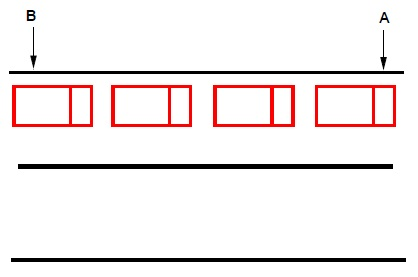
\includegraphics[width=0.7\textwidth]{capitulos/5/figuras/figura1.jpg}
	\caption{\label{fig:densidad} Ilustración de Densidad}	
\end{figure}

\section{Estimación de Tráfico en tiempo real}

Para la estimación de tráfico en tiempo real, los países desarrollados utilizan redes de sensores detectores \cite{leduc2008road} como fuente de datos. Desde el verano de 2007, la Dirección General de Tráfico (DGT) del Ministerio del Interior de España ha estado proveyendo una gran cantidad de datos de tráfico en tiempo real integrados con los mapas de Google. Utilizando unos 4000 sensores de tráfico localizados a lo largo de la red de caminos españoles. Esta herramienta permite, por ejemplo, recolectar el flujo de tráfico por hora y la velocidad promedio en los alrededores de Madrid (\Cref{fig:mapaTrafico}) a través de sensores ubicados en los cruces de las carreteras.

\begin{figure}[h]
	\centering
	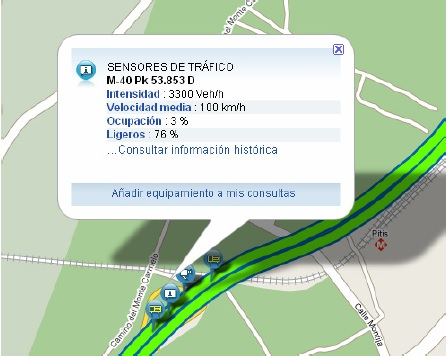
\includegraphics[width=0.7\textwidth]{capitulos/5/figuras/figura2.jpg}
	\caption{\label{fig:mapaTrafico} Típica información proveída por el mapa de tráfico de la DGT}	
\end{figure}

Otros países como Francia, Reino Unido y Portugal cuentan con sistemas similares a los de España. También existen varios estudios basados en FCD para la estimación de tráfico en tiempo real, en \cite{herrera2010evaluation} presentan uno de los primeros experimentos de campo utilizando teléfonos celulares equipados con GPS para obtener datos de tráfico en tiempo real, en el mismo se utilizaron 100 vehículos que llevaban un nokia N95 a bordo. La prueba consistió en conducir en círculos en un tramo de aproximadamente 15 kilómetros de la carretera I-880, cerca de Union City. Los resultados obtenidos del experimento sugerían que una penetración de 2-3\% de teléfonos móviles entre los conductores era suficiente para proveer medidas precisas de la velocidad del flujo de tráfico. En otros trabajos como \cite{reinthaler2007evaluation} se utiliza a taxis como vehículos de prueba para la obtención de FCD, debido a que las medidas de velocidad provenientes de taxis son representativas de la velocidad promedio de toda la población de vehículos \cite{linauer2004fleet}. 

Aparte de la estimación de tráfico, también es posible realizar predicciones del estado del tráfico basándose en la información actual e histórica del tráfico. En \cite{de2008traffic} trabajaron con 600.000 vehículos que enviaban su ubicación cada tres minutos, y a través de dos algoritmos basados en redes neuronales y emparejamiento de patrones realizaban predicciones a corto plazo (15 a 30 minutos) del estado de tráfico futuro. Logrando un error situado entre 2\% a 8\% en predicciones de 15 minutos y 3\% a 16\% para predicciones de 30 minutos.
\chapter{Implementación de la Solución}
\label{cap:6}

En este capítulo se presentan los detalles de implementación de un sistema centralizado cuyo objetivo es aproximar el estado del tráfico en tiempo real. La solución propuesta está basada en FCD obtenido mediante dispositivos móviles. La información resultante es almacenada en una base de datos GIS y se encuentra disponible para consultas a través de una aplicación móvil y una página web desarrolladas para el efecto.

\section{Arquitectura}

En la \Cref{fig:arquitectura} se ilustra la arquitectura modular del sistema desarrollado. La plataforma cuenta con tres componentes principales:
\begin{enumerate*}[1)] \item una base de datos GIS que almacena el mapa de calles y las trayectorias de los vehículos, \item una aplicación móvil que captura los datos del trayecto recorrido por los vehículos y \item una aplicación web que procesa los datos obtenidos y genera información sobre el estado del tránsito.
\end{enumerate*}

\begin{figure}[h]
	\centering
	\input{capitulos/6/figuras/figura61.pdf_tex}
	\caption{\label{fig:arquitectura} Arquitectura del Sistema}	
\end{figure}

Para el almacenamiento de la información se utiliza el motor de base de datos PostgreSQL\footnote{http://www.postgresql.org/} al que además se agregan las extensiones PostGIS\begin{flushright}
	\footnote{http://postgis.net/}
\end{flushright}, que añade capacidades GIS, y pgRouting\footnote{http://pgrouting.org/}, que añade funciones de ruteo geoespacial. Por otro lado, con el propósito de recolectar la información de FCD se cuenta con una aplicación móvil desarrollada para sistemas operativos Android\footnote{http://developer.android.com/index.html} 2.3 o superior, que se ejecuta en los dispositivos de los usuarios. Por último, para el procesamiento y recuperación de la información se cuenta con una aplicación web desarrollada con tecnología Java EE\footnote{http://docs.oracle.com/javaee/} que implementa servicios REST a través de los cuáles la aplicación móvil envía y obtiene datos del servidor.

\section{Almacenamiento de datos}
\label{base-de-datos}

A modo de generar información sobre el estado del tráfico de un área geográfica en particular, se debe contar con un mapa de calles y con un conjunto de trayectorias obtenidas mediante FCD durante un período de tiempo determinado. El mapa y las trayectorias deben estar almacenados en la base de datos GIS para posteriormente ser utilizados durante el procesamiento de la información.

Primeramente, para el mapa de calles se utilizan los datos geográficos disponibles en Open Street Maps\footnote{http://www.openstreetmap.org/} (OSM). Los datos descargados desde OSM están en el formato OSM XML, el cual consiste en una lista de instancias de nodos, caminos y relaciones dentro de su modelo. Antes de almacenar estos datos es necesario transformarlos a un formato soportado por PostGIS y pgRouting. pgRouting representa toda la información de las rutas como un grafo dirigido, donde los vértices corresponden a las intersecciones de las calles y las aristas corresponden a los segmentos de calles, la longitud de la calle determina su peso, que es utilizado para el cálculo del camino más corto. Para convertir e importar los datos de OSM a la base de datos se utiliza la herramienta osm2po\footnote{http://osm2po.de/} y como resultado de esta importación se crea una tabla en la que cada fila corresponde a un segmento de calle. 

Por otro lado, para almacenar la información de las trayectorias de los usuarios se definen las siguientes tablas:
\begin{enumerate}
\item \textbf{Localizaciones}: En esta tabla se guardan los datos de ubicación que son recibidos periódicamente de los usuarios de la aplicación móvil. Se almacena la fecha, la latitud, la longitud, la velocidad, la dirección, la precisión, altitud y la ruta a la que pertenece. Las localizaciones representan los puntos de una trayectoria.
\item \textbf{Rutas}: Una ruta es un conjunto de localizaciones que sirven como dato de entrada para el proceso de MM. La ruta representa a la trayectoria recorrida por el usuario durante un viaje.
\end{enumerate}

Todos los datos geométricos, tanto del mapa de calles como de las trayectorias, son almacenados utilizando un sistema de coordenadas WGS84 conforme se describe en el \cref{sistema_de_coordenadas}.

\section{Implementación de FCD}
\label{floating-car-data}

La información de FCD es obtenida por medio de una aplicación móvil desarrollada como parte del presente trabajo que ha sido denominada Autotracks\footnote{https://play.google.com/store/apps/details?id=py.com.fpuna.autotracks}. La misma se encarga de capturar, almacenar y enviar periódicamente a un servidor central las trayectorias de los usuarios, además la aplicación sólo captura las localizaciones mientras los usuarios están en un vehículo en movimiento. Para este propósito, Autotracks cuenta con tres componentes principales: 
\begin{itemize}
	\item Reconocimiento de actividad.
	\item Toma de localizaciones.
	\item Envío de datos.
\end{itemize}

\subsection{Reconocimiento de actividad}
\label{reconocimiento_actividad}

El reconocimiento de actividad consiste en determinar la acción que está realizando una persona en base a un patrón de movimientos observados para dicha persona, estas actividades pueden ser por ejemplo una caminata, un paseo en bicicleta, etc. Para realizar el reconocimiento de actividad se pueden utilizar los sensores con los que cuentan los dispositivos móviles, como el acelerómetro, el giroscopio y los dispositivos GPS integrados. En Autotracks se utiliza el reconocimiento de actividad para determinar cuando un usuario se encuentra en un vehículo en movimiento.

En \cite{liao2006location,bao2004activity,ravi2005activity} se describen técnicas que permiten detectar la actividad mediante los sensores GPS y el acelerómetro de los dispositivos móviles. En \cite{thiagarajan2010cooperative} se utilizan estas técnicas de reconocimiento de actividad para determinar si el usuario está en un vehículo en movimiento. En Autotracks, en lugar de implementar un algoritmo de reconocimiento de actividad propio, se reutiliza una implementación proveída como parte de Google Play Services\footnote{http://developer.android.com/google/play-services/index.html}, denominada Activity Recognition\footnote{http://developer.android.com/training/location/activity-recognition.html}, que permite detectar distintos tipos de actividad del usuario, por ejemplo si está en un vehículo, en bicicleta, caminando, corriendo, o si está totalmente quieto.

Autotracks consulta periódicamente la actividad del usuario, cuando se ha detectado que el usuario se encuentra en un vehículo en movimiento se inicia el servicio de toma de localizaciones, este servicio permanece activo mientras el usuario se encuentra en movimiento. Para detectar la actividad del usuario se utiliza un intervalo de 30 segundos. Una vez que se ha detectado que el usuario ya no está en movimiento durante más de 10 minutos, el servicio de toma de localizaciones es detenido. Se utiliza la tolerancia de 10 minutos para evitar que el servicio se detenga cuando el vehículo se encuentra momentáneamente detenido en espera de algún evento, como en un semáforo en rojo, esperando por alguna persona o en un embotellamiento. Los valores previamente mencionados fueron determinados y ajustados empíricamente.

El \Cref{alg:deteccion_actividad} muestra el procedimiento ejecutado periódicamente cada vez que se obtiene un resultado del reconocimiento de actividad. Este procedimiento verifica si la toma de localizaciones está o no iniciada y se encarga de iniciarla o finalizarla de acuerdo a la actividad detectada. El resultado de la detección es almacenado para ser utilizado en la siguiente invocación del procedimiento. Si se ha detectado que el usuario está en un vehículo, el tiempo en el que ocurrió la detección también es almacenado para utilizarlo en la siguiente invocación. En el sub-procedimiento $\Call {EstaEnVehiculo}{}$, si el usuario está a pie se detiene inmediatamente el rastreo, si está en un vehículo se continúa con el rastreo, y en cualquier otro caso (está en bicicleta, o quieto, o no se pudo determinar la actividad) se verifica el estado anterior de movimiento y el tiempo de la última detección de movimiento antes de tomar una decisión.
 
\begin{algorithm}
\caption{Procedimientos de Reconocimiento de Actividad}
\label{alg:deteccion_actividad}
\begin{algorithmic}[1]
\Procedure{ActividadDetectada}{$actividad$}
	\State $enVehiculo =$ \Call {EstaEnVehiculo}{$actividad$}
%	\State Guardar $enVehiculo$ como el último estado detectado  
	\If {$enVehiculo$}
		\State $ultimoEstado = \text{EN\_VEHICULO}$
		\If {RASTREO no está iniciado}
			\State Iniciar RASTREO
		\EndIf
	\Else
		\State $ultimoEstado = null$
		\If {RASTREO está iniciado}
			\State Finalizar RASTREO
		\EndIf
	\EndIf
\EndProcedure
\Statex
\Function {EstaEnVehiculo}{$actividad$}
	\If {$actividad == \text{A\_PIE}$}
		\State \Return $falso$
	\Else
		\State Inicializar $t$ al tiempo actual
		\If {$actividad == \text{EN\_VEHICULO}$}
			\State $t\_ultimaDeteccion = t$ 
			\State \Return $verdadero$
		\Else
		\If {$ultimoEstado == \text{EN\_VEHICULO}$}
			\State $\Delta t = t - t\_ultimaDeteccion$
			\If {$\Delta t \leq$ TOLERANCIA}
				\State \Return $verdadero$
			\Else
				\State \Return $falso$
			\EndIf
		\Else
			\State \Return $falso$
		\EndIf
		\EndIf
	\EndIf
\EndFunction
\end{algorithmic}
\end{algorithm}

\subsection{Toma de localizaciones}
\label{toma_localizaciones}

Para obtener la ubicación de los teléfonos móviles existen varias opciones posibles, cada una con sus ventajas y desventajas, estas son: 
\begin{itemize}
\item \textbf{Triangulación de antenas}: Utiliza las antenas de telefonía para determinar la posición. Requiere un uso mínimo de batería pero produce resultados de baja precisión, dependiendo de la técnica utilizada la precisión varía de 50 a 200 metros en áreas urbanas, y hasta más de 2 kilómetros en zonas suburbanas.
\item \textbf{WiFi}: Utiliza las posiciones conocidas de los puntos de acceso Wifi para estimar la ubicación. El uso de la batería es moderado y produce resultados con una precisión de menos de 50 metros. No es apropiado para zonas rurales donde existe una escasa cantidad de puntos de acceso Wifi de referencia.
\item \textbf{GPS}: Utiliza la red de satélites GPS para obtener la posición del dispositivo. Este mecanismo requiere un alto consumo de batería y su precisión es de menos de 10 metros en el mejor caso. La precisión disminuye considerablemente cuando se pierde la visibilidad de los satélites.
\end{itemize}
A fin de tener la mayor flexibilidad posible, Autotracks es capaz de trabajar con cualquiera de estas opciones para obtener la ubicación de los dispositivos. Para ello se reutiliza una implementación denominada \emph{Fused Location Provider}\footnote{http://developer.android.com/training/location/receive-location-updates.html} que está disponible como parte \emph{Google Play Services}.

En los casos en los que la localización es obtenida a través de las redes GSM o WiFi no se dispone de la información de velocidad, la cual es necesaria para el procesamiento posterior. Para paliar esta falta de información, la velocidad es estimada utilizando la localización anterior de la siguiente manera: \begin{equation} \label{eq:velocidad} v=\frac { d }{ t } \end{equation} donde $d$ es la distancia entre la localización actual y la anterior, y $t$ es el tiempo que transcurrió entre la toma de las localizaciones.

Algunas de las localizaciones capturadas pueden llegar a ser demasiado imprecisas como para ser utilizadas en el procesamiento posterior. Para evitar este tipo de localizaciones erróneas se utilizan dos técnicas de filtrado. El primer método consiste simplemente en descartar las localizaciones que reportan una precisión mayor a 200 metros. El segundo método consiste en determinar la velocidad a la que tuvo que haber viajado el vehículo para pasar de la posición anterior a la posición actual utilizando la \cref{eq:velocidad}, si dicha velocidad es mayor a un valor preestablecido, en este caso de 140 km/h, la localización es descartada. Además, también se descartan las localizaciones que son muy próximas entre sí debido a que el algoritmo de MM utilizado en una siguiente etapa requiere que las localizaciones sean relativamente distantes entre sí. Los valores de referencia fueron determinados empíricamente en sucesivas pruebas de campo. En el \Cref{alg:toma_de_localizaciones} se describe el procedimiento utilizado para registrar una localización.

\begin{algorithm}
	\caption{Toma de Localizaciones}
	\label{alg:toma_de_localizaciones}
	\begin{algorithmic}[1]
		\Procedure {Registrar}{$localizacion$}
		\State $esValida = \Call{EsValida}{localizacion}$
		\If {$esValida$}
		\State $ultimaLocalizacion = localizacion$
		\EndIf
		\EndProcedure
		\Statex
		\Function {EsValida}{$localizacion$}
		\State Inicializar $p$ a la precisión de la $localizacion$	
		\State $\Delta d = \Call{Distancia}{localizacion, ultimaLocalizacion}$
		\State $\Delta t = \Call{Tiempo}{localizacion, ultimaLocalizacion}$
		\State $v = \Delta d / \Delta t$
		\If {$\Delta d > \text{D\_MIN} \land v < \text{V\_MAX} \land p < \text{P\_MAX}$}
		\State \Return $verdadero$
		\Else
		\State \Return $falso$
		\EndIf
		\EndFunction
	\end{algorithmic}
\end{algorithm}

Otro aspecto importante a tener en cuenta es la frecuencia con la que se toman las localizaciones. En \cite{tao2012real} se sugiere que intervalos de entre 10 y 20 segundos son los recomendados en aplicaciones prácticas. En \cite{fontaine2005part} se reivindica que intervalos de muestras más largos permiten obtener información sobre mayores distancias y reduce la probabilidad de capturar velocidades no representativas. En \cite{lou2009map,giovannini2011novel} se utilizan localizaciones con intervalos de más de 3 minutos en aplicaciones \emph{off-line}. Para lograr un balance entre la frecuencia y el consumo de batería, se establece un intervalo de 60 segundos para el muestreo utilizado en Autotracks, dicho valor también fue determinado empíricamente realizando pruebas de campo en dispositivos de diversa gama.

\subsection{Envío de datos}

La aplicación envía los datos de las localizaciones a través de Internet a un servidor central que se encarga de almacenar y procesar la información. Para disminuir el consumo de batería ocasionado por la utilización de la red de datos móviles, los teléfonos almacenan temporalmente las localizaciones capturadas y las envían periódicamente al servidor. Luego de que un grupo de localizaciones ha sido enviado es borrado de la memoria del teléfono.

El intervalo de tiempo definido para el envío de los datos es de 15 minutos. Para disminuir el consumo de batería se utiliza el mecanismo de alarmas inexactas proveído por Android\footnote{https://developer.android.com/training/scheduling/alarms.html}. Al utilizar este tipo de alarmas, el sistema operativo sincroniza las alarmas de múltiples aplicaciones y las dispara al mismo tiempo. Esto reduce el número total de veces que el sistema debe despertar el dispositivo, reduciendo así el uso de la batería.

Para enviar las localizaciones no es necesario que el usuario haya finalizado completamente su recorrido, al momento de dispararse una alarma todas las localizaciones capturadas hasta el momento son enviadas al servidor. El resto de las localizaciones del mismo recorrido son enviadas al dispararse las siguientes alarmas. De esta forma los recorridos parciales pueden ser utilizados para estimar el estado del tráfico aproximadamente en tiempo real.

\section{Implementación de MM}
\label{implementacion_mm}

Un proceso de Map Matching (MM) es ejecutado cada vez que las trayectorias de los vehículos son enviadas desde los teléfonos móviles al servidor central para determinar el camino real recorrido por cada vehículo. Para realizar este proceso se utiliza el algoritmo propuesto por \cite{lou2009map}, conocido como ST-Matching, con las mejoras propuestas por \cite{budigm2012algorithm} y \cite{sakic2012map}. 

ST-Matching es un algoritmo topológico específicamente diseñado para funcionar de forma \emph{off-line} y con intervalos de tiempo relativamente largos entre las muestras. Su implementación es sencilla comparada con otras técnicas avanzadas como \cite{quddus2006high, newson2009hidden} y no requiere de procesamientos y cálculos matemáticos complejos. Estas características se adecuan a los requerimientos impuestos por la arquitectura de la solución propuesta. 

El algoritmo ST-Matching consta de tres partes principales: \begin{enumerate*}[a)]
\item la \emph{Selección de Candidatos},
\item el \emph{Análisis Espacial y Temporal} y
\item la \emph{Obtención del Resultado}.
\end{enumerate*}
La \Cref{fig:st-matching} muestra una descripción general del proceso cuyo resultado es almacenado en la base de datos para ser utilizado más adelante en el análisis de tráfico.

\begin{figure}[h]
	\centering
	\input{capitulos/6/figuras/figura62.pdf_tex}
	\caption[Descripción General de ST-Matching]{Descripción general del algoritmo ST-Matching.}
	\label{fig:st-matching} 
\end{figure}

\subsection{Marco conceptual base para MM}

Los datos de entrada del algoritmo de MM son la red de calles, que se describió en el \cref{base-de-datos}, y la trayectoria de un vehículo, obtenida mediante el uso de la aplicación móvil, como se explica en el \cref{floating-car-data}. El resultado de este procesamiento es una aproximación del camino real recorrido por el vehículo.

La red de calles es modelada como un grafo dirigido $G(V,E)$, donde $V$ es el conjunto de todos los vértices correspondientes a las intersecciones y extremos de los segmentos de calles, y $E$ es el conjunto de todas las aristas que representan segmentos de calles. Además, cada segmento $e \in E$ tiene como datos un identificador único $e.id$, el límite de velocidad $e.v$ de la calle, la longitud $e.l$ del segmento, el identificador del vértice inicial $e.ini$ y el del vértice final $e.fin$. En la \Cref{fig:segmentos_de_calle} se aprecia como una calle puede estar dividida en varios segmentos, donde cada segmento está comprendido entre dos vértices del mapa.

\begin{figure}[h*]
	\centering
	\input{capitulos/6/figuras/figura63.pdf_tex}
	\caption{\label{fig:segmentos_de_calle} Representación de segmentos de calles}	
\end{figure}

La trayectoria $T$ de un vehículo es representada como una secuencia ordenada de puntos $p_1, p_2, \dots, p_n$ donde cada punto $p_i$ tiene además como datos su latitud $p.lat$, su longitud $p.lon$, su velocidad aproximada $p.v$, su dirección de desplazamiento $p.d$ y el tiempo $p.t$ en que fue tomada la muestra. La trayectoria está ordenada con respecto al tiempo de tal manera que $p_i.t < p_{i + 1}.t$ para $1 \le i < n$. La \Cref{fig:trayectoria} muestra un ejemplo de una trayectoria correspondiente a un vehículo de prueba.

\begin{figure}[h*]
	\centering
	\input{capitulos/6/figuras/figura64.pdf_tex}
	\caption{\label{fig:trayectoria} Trayectoria de un vehículo}	
\end{figure}

El camino real $R$ es definido como una secuencia de segmentos de calles $e_i$ conectados entre sí, que se inicia en un vértice $v_{ini} \in V$ y finaliza en un vértice $v_{fin} \in V$, es decir, $R = \{ e_1, e_2, \dots, e_n \}$, donde $e_1.ini = v_{ini}$, $e_n.fin = v_{fin}$ y $e_i.fin = e_{i + 1}.ini$ para $1 \le i < n$.

En base a estas definiciones, el problema de MM se puede expresar de la siguiente forma: \emph{Dada una trayectoria T y una red de calles G(V,E), encontrar el camino real R que hace coincidir a T con su reconstrucción más realista sobre G(V,E).}

\subsection{Selección de Candidatos}
\label{seleccion_de_candidatos}

La primera etapa del proceso es la selección de puntos candidatos. Un punto candidato $c$ es un punto perteneciente a un segmento de calle $e$, que puede formar parte del camino real recorrido por un vehículo, y que es obtenido a partir de un punto $p$ de una trayectoria. Dada una trayectoria $T = \{p_1, p_2, \dots, p_n\}$, el proceso de selección de candidatos consiste en encontrar para cada punto $p_i$, $1\le i\le n$, el conjunto de puntos candidatos $C_i = \{c_{i}^{1}, c_{i}^{2}, \dots, c_{i}^{m}\}$ correspondiente.

El primer paso es seleccionar todos los segmentos de calles $e \in E$ tales que la distancia entre un punto $p_i$ y un segmento $e$ sea menor a un radio $r$, de esta forma se obtiene un conjunto de segmentos $E_i = \{ e : \text{ } e \in E \text{ } \wedge \text{ } dist(p_i, e) < r \}$. Luego, para cada segmento $e_{i}^{j}$ perteneciente al conjunto $E_i = \{e_{i}^{1}, e_{i}^{2}, \dots, e_{i}^{m}\}$ resultante, se obtiene un punto candidato $c_{i}^{j}$ realizando una proyección del punto $p_i$ sobre el segmento $e_{i}^{j}$. La proyección $proy(p, e)$ de un punto $p$ sobre un segmento $e$ se define como el punto $c$ perteneciente a $e$ más cercano a $p$, es decir, $c = \text{arg } min(dist(c_i, p)) \text{ } \forall c_i \in e$. Así, se obtiene el conjunto de puntos candidatos $C_i = \{ proy(p_i, e_j) \text{ } \forall e_j \in E_i \}$. Como se puede apreciar en la \Cref{fig:puntos_candidatos} un punto candidato puede ser cualquier punto del segmento, como en el caso de $c_{i}^{1}$ y $c_{i}^{2}$, o uno de sus vértices como en el caso de $c_{i}^{3}$.

\begin{figure}[h*]
	\centering
	\input{capitulos/6/figuras/figura65.pdf_tex}
	\caption{\label{fig:puntos_candidatos} Puntos candidatos para un punto de la trayectoria}	
\end{figure}

Para la obtención de cada conjunto $C_i$ se ejecuta la \Cref{lst:candidatos}, donde los comandos precedidos por el prefijo \emph{ST\_} son funciones espaciales implementadas por PostGIS. Utilizando \emph{ST\_DWithin} se obtienen todos los segmentos de calle que se encuentren a una distancia menor o igual a un radio $r$ del punto observado $p$. Luego, el punto observado es proyectado sobre cada segmento de calle utilizando \emph{ST\_LineLocatePoint} y \emph{ST\_LineInterpolatePoint} para obtener el punto candidato correspondiente.

\begin{lstlisting}[float,floatplacement=!htb,caption={Selección de puntos candidatos}, label={lst:candidatos}]
-- geom es la geometria del punto p
-- dist es el radio r de consideracion
select pgr.id,     -- identificador del segmento de calle 
       pgr.source, -- identificador del nodo inicial
       pgr.target, -- identificador del nodo final
       pgr.km,     -- longitud del segmento de calle
       pgr.kmh,    -- limite de velocidad del segmento
       pgr.x1,     -- longitud del nodo inicial
       pgr.y1,     -- latitud del noto inicial
       pgr.x2,     -- longitud del nodo final
       pgr.y2,     -- latitud del nodo final
       ST_X(point) as lon, -- longitud del punto proyectado
       ST_Y(point) as lat  -- latitud del punto proyectado
from (
    select 
        pgr.*,  -- datos del segmento de calle 
        ST_LineInterpolatePoint(
            geom_way, 
            ST_LineLocatePoint(
                geom_way, 
                :geom
            )
        ) as point -- punto proyectado
    from asu_2po_4pgr as pgr
    where ST_DWithin(:geom, geom_way, :dist)
) a
\end{lstlisting}

Una vez que se han obtenidos todos los conjuntos $C_i = \{c_{i}^{1}, c_{i}^{2}, \dots, c_{i}^{m}\}$ correspondientes a cada punto $p_i$ de la trayectoria $T$, el problema de MM se reduce a cómo seleccionar un punto candidato $c_i$ de cada conjunto $C_i$, a partir del cual se obtiene el segmento de calle $e_i$, de manera tal que el camino real resultante $R = \{ e_1, e_2, \dots, e_n \}$ sea lo más aproximado posible a $T = \{ p_1, p_2, \dots, p_n\}$, conforme se describe en los siguientes apartados.

\subsection{Análisis Espacial y Temporal}

La segunda etapa del proceso tiene por objetivo seleccionar el punto candidato $c_i$ de cada conjunto $C_i$ que sea el más apropiado para cada punto $p_i$ de la trayectoria. Para ello cada punto candidato y cada posible conexión entre dos puntos candidatos consecutivos son analizados de acuerdo a dos criterios de calidad, el \emph{análisis espacial} y el \emph{análisis temporal}.

\subsubsection{Análisis Espacial}

En el análisis espacial se utiliza información geométrica y topológica de la red de calles para evaluar los puntos candidatos. La información geométrica es incorporada utilizando la \emph{probabilidad de observación} y la información topológica es expresada utilizando la \emph{probabilidad de transmisión}.

La \emph{probabilidad de observación} es la probabilidad de que un punto candidato $c_{i}^{j}$ corresponda a un punto $p_i$ de la trayectoria, calculada en base a la distancia $dist(c_{i}^{j},p_i)$ entre los puntos. Asumiendo que el error en la medición de la posición de $p_i$ sigue una distribución normal, la probabilidad de observación $N(c_{i}^{j})$ se define como
\begin{equation} \label{probabilidad_de_observacion}
N(c_{i}^{j}) = \frac {1}{\sqrt { 2 \pi \sigma }} {e}^{\frac {{(x_{i}^{j} - \mu)}^{2}}{{ 2 \sigma}^{2}}}
\end{equation}
donde $x_{i}^{j} = dist(c_{i}^{j},p_i)$ es la distancia entre $p_i$ y el punto candidato $c_{i}^{j}$. En este trabajo se utiliza una media $\mu = 50\text{m}$ y una desviación estándar $\sigma = 100\text{m}$. Estos valores fueron determinados empíricamente y son distintos a los valores utilizados en \cite{lou2009map} y \cite{budigm2012algorithm} debido a que, a diferencia de estos trabajos anteriores, no todas las muestras son obtenidas mediante el uso de GPS.

El cálculo de la probabilidad de observación tiene en cuenta únicamente la posición de los puntos $p_i$ y $c_{i}^{j}$, ignorando la topología y la posición relativa de los puntos con respecto a los demás puntos de la trayectoria. Debido a esto pueden darse casos en los que un punto candidato es seleccionado erróneamente por ser el más cercano aún cuando existen otros puntos candidatos más adecuados. Esta situación se puede presentar en las intersecciones de calles o en calles paralelas muy cercanas como se muestra en la \Cref{fig:probabilidad_transmision}.

\begin{figure}[h*]
	\centering
	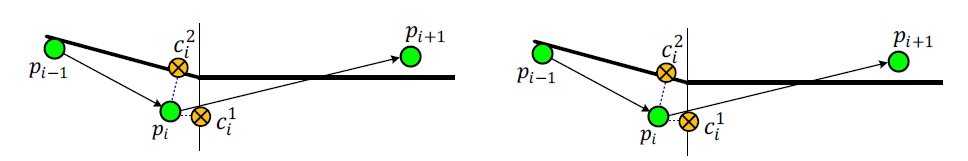
\includegraphics[width=0.9\textwidth]{capitulos/6/figuras/figura7.jpg}
	\caption{\label{fig:probabilidad_transmision} Errores en la probabilidad de observación}	
\end{figure}

Para minimizar la ocurrencia de estos problemas se introduce un segundo criterio denominado \emph{probabilidad de transmisión}, que se define como la probabilidad de que el camino más corto entre un punto candidato $c_{i-1}^{j}$ y el siguiente punto candidato $c_{i}^{k}$ es el camino correcto de $p_{i-1}$ a $p_i$. La probabilidad de transmisión se calcula de la siguiente forma: 
\begin{equation} \label{probabilidad_de_transmision}
V(c_{i-1}^{j}, c_{i}^{k}) = \frac { min( dist(p_{i-1}, p_i), long(c_{i-1}^{j}, c_{i}^{k})) }{ max (dist(p_{i-1}, p_i), long(c_{i-1}^{j}, c_{i}^{k})) }
\end{equation}
donde $long(c_{i-1}^{j}, c_{i}^{k})$ es la longitud del camino más corto entre $c_{i-1}^{j}$ y $c_{i}^{k}$. El cálculo del camino más corto se realiza utilizando el algoritmo de Dijkstra\footnote{http://es.wikipedia.org/wiki/Algoritmo\_de\_Dijkstra} para grafos dirigidos. La dirección de las aristas del grafo representan el sentido de circulación de la calle, de esta forma se incorpora información topológica en el análisis espacial. 

Combinando la \Cref{probabilidad_de_observacion} y la \Cref{probabilidad_de_transmision} se define la función de análisis espacial $F_s(c_{i-1}^{j},c_{i}^{k})$ como el producto de la probabilidad de observación y la probabilidad de transmisión de la siguiente forma:
\begin{equation} \label{funcion_espacial}
F_s(c_{i-1}^{j},c_{i}^{k}) = N(c_{i}^{k}) \times V(c_{i-1}^{j}, c_{i}^{k}), \quad 2 \le i \le n 
\end{equation}

Como resultado del análisis espacial se asigna un valor numérico a todos los posibles caminos que van de $p_{i-1}$ a $p_i$ obtenido mediante la \Cref{funcion_espacial}.

\subsubsection{Análisis Temporal}

Existen casos en los que el análisis espacial no es suficiente para identificar un segmento de calle correctamente. En la \Cref{fig:analisis_temporal} la línea más gruesa representa a una autopista mientras que la línea más delgada representa a una calle vecinal, el límite de velocidad de la autopista es superior al de la calle vecinal cercana, utilizando sólo el análisis espacial se podría seleccionar incorrectamente una de las dos. Para evitar esto se calcula la velocidad promedio entre dos puntos consecutivos $p_{i-1}$ y $p_i$ y se compara con los límites de velocidad promedio de los segmentos de calles comprendidos entre dos puntos candidatos $c_{i-1}^{j}$ y $c_{i}^{k}$ con el fin de seleccionar el segmento cuya velocidad promedio es la más cercana a la velocidad promedio de desplazamiento del vehículo.

\begin{figure}[h*]
	\centering
	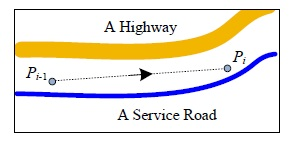
\includegraphics[width=0.6\textwidth]{capitulos/6/figuras/figura8.jpg}
	\caption{\label{fig:analisis_temporal} Error en el análisis espacial}	
\end{figure}

Dados dos puntos candidatos $c_{i-1}^{j}$ y $c_{i}^{k}$ correspondientes a dos puntos consecutivos $p_{i-1}$ y $p_i$ respectivamente, el camino más corto entre $c_{i-1}^{j}$ y $c_{i}^{k}$ es una lista de segmentos $[e_1, e_2, \dots, e_n]$. La velocidad promedio de desplazamiento del vehículo en este camino más corto se define como:
\begin{equation}
\overline{v} = \frac { \sum_{m=1}^{n} {e_m.l} }{ \Delta t_{i-1, i} }
\end{equation}
donde $e_m.l$ es la longitud del segmento $e_m$ y $\Delta t_{i-1, i} = p_i.t - p_{i-1}.t$ es el intervalo de tiempo entro dos puntos consecutivos de la trayectoria. Además, cada segmento $e_m$ tiene una velocidad $e_m.v$ correspondiente al límite de velocidad de la calle. La Similaridad Coseno\footnote{http://es.wikipedia.org/wiki/Similitud\_coseno} es utilizada para medir la semejanza entre $\overline{v}$ y los límites de velocidad. De esta forma, la función de análisis temporal queda definida así:
\begin{equation} \label{funcion_temporal}
F_{ t }(c_{ i-1 }^{ j },c_{ i }^{ k })=\frac { \sum _{ m=1 }^{ n }{ (e_{ m }.v\times \overline { v } ) }  }{ \sqrt { \sum _{ m=1 }^{ n }{ (e_{ m }.v)^{ 2 } }  } \times \sqrt { \sum _{ m=1 }^{ n }{ (\overline { v } )^{ 2 } }  }  } 
\end{equation}

\subsection{Búsqueda del Resultado}

\label{busqueda_de_resultado}
El resultado de los procesos descritos anteriormente es un grafo acíclico dirigido de puntos candidatos, que representa todos los posibles caminos entre el punto inicial $p_1$ y el punto final $p_n$ de la trayectoria $T$. Como se muestra en la \Cref{fig:grafo_de_candidatos}, los nodos del grafo corresponden a los candidatos de cada punto $p_i$ y las aristas representan los caminos más cortos entre cada par de candidatos $c_{i-1}^j$ y $c_i^k$ consecutivos. A cada arista se le asigna un peso de acuerdo a la probabilidad de transmisión entre su vértice inicial y final, y a la probabilidad de observación del vértice inicial.

\begin{figure}[h*]
	\centering
	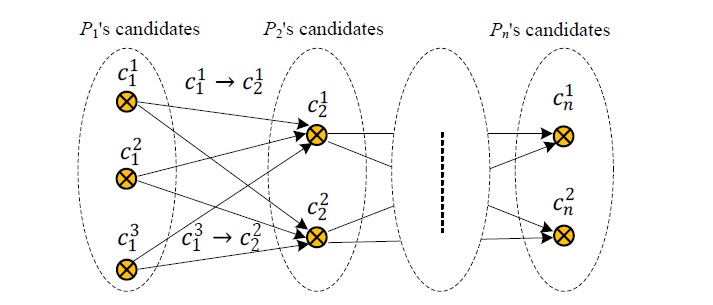
\includegraphics[width=0.9\textwidth]{capitulos/6/figuras/figura9.jpg}
	\caption{\label{fig:grafo_de_candidatos} Grafo de puntos candidatos}	
\end{figure}

Para asignar el peso a cada arista se combinan la \cref{funcion_espacial} y la \cref{funcion_temporal} definiendo así la función espacio-temporal de la siguiente forma:
\begin{equation} \label{funcion_espacio_temporal}
F(c_{i-1}^{j},c_{i}^{k}) = F_s(c_{i-1}^{j},c_{i}^{k}) \times F_{ t }(c_{ i-1 }^{ j },c_{ i }^{ k }), 2 \leq i \leq n
\end{equation}

Dada una secuencia de puntos candidatos $C_T = \{c_1, c_2, \dots, c_n\}$, el peso global se define como $F(C_T) = \sum _{ i=2 }^{ n }{F(c_{i-1}^{j},c_{i}^{k})}$, es decir, es la sumatoria de los pesos de todas las aristas que componen la secuencia. El objetivo del algoritmo es obtener la secuencia que tenga el mayor peso.

El \Cref{alg:st_matching} muestra los pasos realizados para obtener la secuencia de puntos candidatos. El primer paso es construir el grafo $G_T$ de puntos candidatos. Para ello se obtienen todos los conjuntos de puntos candidatos $C_i$ correspondientes a cada punto $p_i$ de la trayectoria $T$. El siguiente paso, es la obtención del resultado final. Primeramente se asigna a todos los candidatos del primer conjunto $C_1$ el valor de su probabilidad de observación $N(c_i^k)$. Luego, para los demás conjuntos $C_i$, se obtienen los valores de la función espacio-temporal para cada par de candidatos consecutivos $c_{i-1}^j$ y $c_i^k$, y para cada $c_i^k$ se guarda el punto candidato previo $c_{i-1}^j$ cuyo valor acumulado sea el mayor. Finalmente se selecciona un punto candidato $c_n^k$ del último conjunto $C_n$, que tenga el valor acumulado más alto y se obtienen todos los puntos candidatos que conforman el camino.

\begin{algorithm}
\caption{ST-Matching}
\label{alg:st_matching}
\begin{algorithmic}[1]
\Procedure {STMatching}{$G:$ grafo de calles, $T:$ trayectoria}
	\State $G_T = \Call{ObtenerCandidatos}{G,T}$
	\State $R = \Call{ObtenerResultado}{G_T}$
	\State \Return $R$
\EndProcedure
\Statex
\Function {ObtenerCandidatos}{$G:$ grafo de calles, $T:$ trayectoria}
	\State Inicializar $G_T$ a un conjunto vacío
	\For {$p_i \in T, 1 \leq i \leq n$} 
		\State $C_i = SeleccionarCandidatos(p_i, G)$
		\State Agregar $C_i$ a $G_T$
	\EndFor
	\State \Return $G_T$
\EndFunction
\Statex
\Function {ObtenerResultado}{$G_T:$ grafo de candidatos}
	\State Definir $f[]$ como el máximo peso computado hasta ahora
	\State Definir $pre[]$ como el padre del punto candidato actual
	\ForAll {$c_1^k$}
		\State $f[c_1^k] = N(c_1^k)$
	\EndFor
	\For {$2 \leq i \leq n$}
		\ForAll {$c_i^k$}
			\State $max = -\infty$
			\ForAll {$c_{i-1}^j$}
				\State $tmp = f[c_{i-1}^j] + F(c_{i-1}^j,c_i^k)$
				\If {$tmp > max$}
					\State $max = tmp$
					\State $pre[c_i^k] = c_{i-1}^j$
				\EndIf
				\State $f[c_i^k] = max$
			\EndFor
		\EndFor
	\EndFor
	\State Inicializar $C$ a una lista vacia de candidados
	\State $c = arg \text{ } max(f[c_n^j])$
	\For {$2 \leq i \leq n$}
		\State Agregar $c$ a $C$
		\State $c = pre[c]$
	\EndFor
	\State Agregar $c$ a $C$
	\State Invertir $C$
	\State \Return $C$
\EndFunction
\end{algorithmic}
\end{algorithm}

\section{Estimación del tráfico}
\label{estimacion_trafico}

Una vez finalizado el proceso MM, a cada punto de la trayectoria se le asocia una arista del mapa de calles por la cual se ha determinado que el vehículo transitó en ese momento. Además cada punto de la trayectoria tiene como dato la velocidad a la cual el vehículo se desplazó. Para realizar la estimación del estado del tráfico se utilizan todas las velocidades de los puntos asociados a cada segmento de calle del mapa durante un período de tiempo determinado.

La estimación se realiza calculando la \emph{velocidad media local} de cada segmento de calle. Para ello se define la velocidad media en la calle $j$ durante el intervalo de interés como:
\begin{equation}
\label{eq:velocidad_media}
{ V }_{ ave }^{ j }({ t }_{ k },{ t }_{ k+\Delta T })=\frac { 1 }{ { n }_{ { t }_{ k },{ t }_{ k+\Delta T } }^{ j } } \sum_{ k={ t }_{ k } }^{ { t }_{ k+\Delta T } }{ \hat { { v } } _{ j }(k) }
\end{equation}
donde ${ \hat { { v } } _{ j }(k) }$ es la velocidad estimada en la calle $j$ durante el intervalo $\left[ { t }_{ k },{ t }_{ k+\Delta T } \right] $, y ${ { n }_{ { t }_{ k },{ t }_{ k+\Delta T }}}$ es el número total de muestras disponibles para la calle $j$ durante dicho intervalo.

Para obtener el estado estimado del tráfico en un momento dado, se utiliza la \Cref{lst:trafico} que da como resultado todos los segmentos de calle $A_iB_i$ formados por los puntos $A_i(r.x1, r.y1)$ y $B_i(r.x2, r.y2)$ junto con la cantidad de muestras disponibles y la sumatoria de las velocidades observadas en dichas muestras durante un periodo de tiempo determinado. Con ello se aplica la \Cref{eq:velocidad_media} para estimar la \emph{velocidad media local} de cada segmento de calle.

\begin{lstlisting}[float,floatplacement=tbh,caption={Obtención de datos de tráfico}, label={lst:trafico}]
select 
    pgr.x1,            -- longitud del nodo inicial
    pgr.y1,            -- latitud del nodo inicial
    pgr.x2,            -- longitud del nodo final
    pgr.y2,            -- latitud del nodo final
    count(l.id),     -- cantidad de muestras observadas
    sum(l.velocidad) -- sumatoria de velocidades observadas
from localizacion as l, asu_2po_4pgr as pgr
where l.wayId = r.id and l.fecha between :inicio and :fin
group by r.id
\end{lstlisting}

Finalmente, para representar la información obtenida en intervalos que faciliten su interpretación, se definen cuatro posibles niveles de velocidad en una calle:
\begin{enumerate}
\item \textbf{Rojo:}  para velocidades entre 0 y 14 kilómetros por hora.
\item \textbf{Naranja:}  para velocidades entre 15 y 29 kilómetros por hora.
\item \textbf{Amarillo:}  para velocidades entre 30 y 39 kilómetros por hora.
\item \textbf{Verde:}  para velocidades de 40 o más kilómetros por hora.
\end{enumerate}
Las calles son pintadas en el mapa de acuerdo a su nivel de velocidad como se puede apreciar en la \Cref{fig:calles}.
\begin{figure}[h]
	\centering
	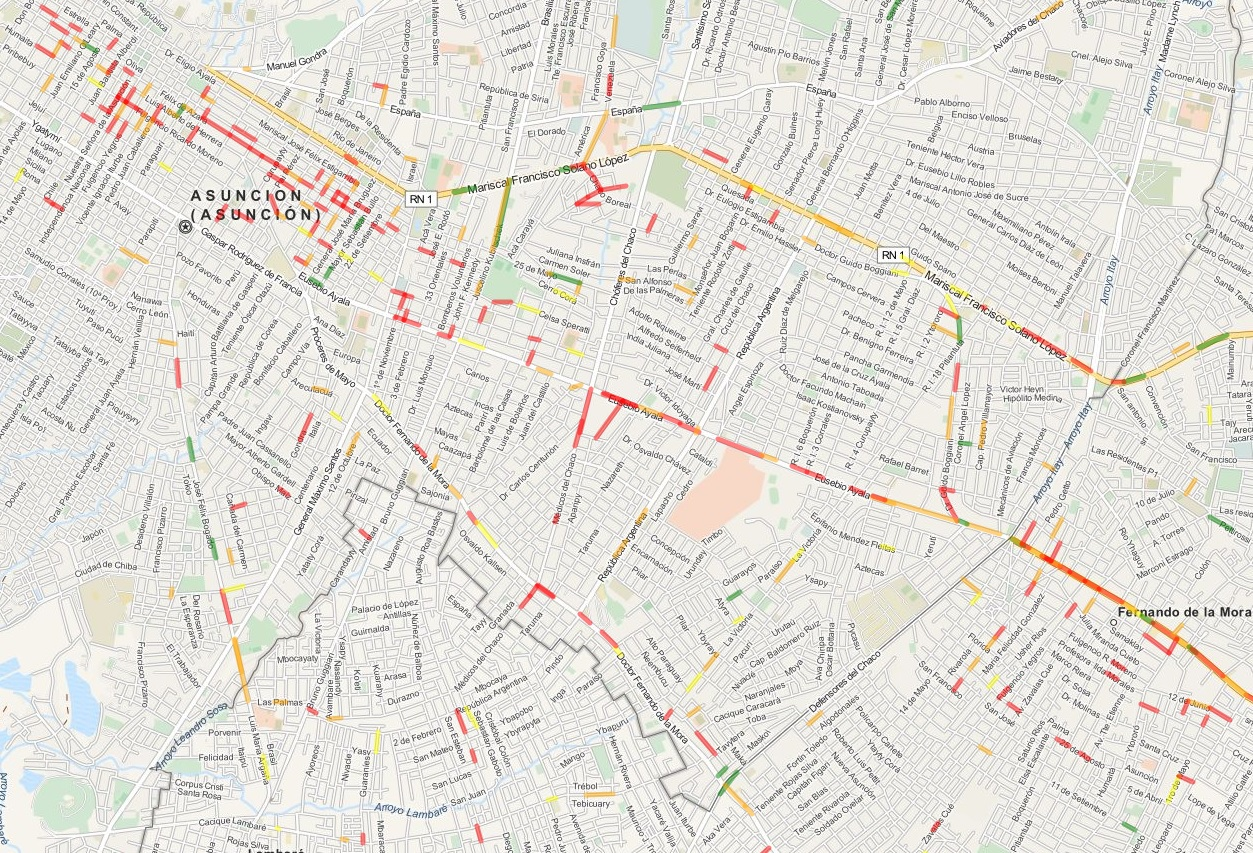
\includegraphics[width=0.7\textwidth]{capitulos/6/figuras/figura3.jpg}
	\caption{\label{fig:calles} Estado de calles en Autotracks}	
\end{figure}

\bibliography{referencias}

\end{document} 